
% ============================================================
%  FLBL2: Layer 2 Blockchain-Based Federated Learning
%  Q1 Journal Rewrite (2026)
% ============================================================

\documentclass{llncs}

\usepackage[T1]{fontenc}
\usepackage{graphicx}
\usepackage{amsmath,amssymb}
\usepackage{tikz}
\usepackage{pgfplots}
\usepackage{xcolor}
\usepackage{booktabs}
\usepackage{array}
\usepackage{multirow}
\usepackage{tabularx}
\usepackage{hyperref}
\usepackage{algorithm}
\usepackage{algpseudocode}
\usepackage{enumitem}
\usepackage[capitalise,noabbrev]{cleveref}
\usepackage{placeins}
\usepackage{rotating}

% Float placement – prevent figures drifting past section end
\renewcommand{\topfraction}{0.90}
\renewcommand{\bottomfraction}{0.80}
\renewcommand{\textfraction}{0.07}
\renewcommand{\floatpagefraction}{0.70}
\setcounter{topnumber}{4}
\setcounter{bottomnumber}{2}
\setcounter{totalnumber}{6}

\pgfplotsset{compat=1.18}
\usepgfplotslibrary{fillbetween}
\usetikzlibrary{arrows.meta,positioning,shapes.geometric,fit,backgrounds,calc}

% Colour palette
\definecolor{clrEdge}{RGB}{0,114,178}
\definecolor{clrAgg}{RGB}{213,94,0}
\definecolor{clrIPFS}{RGB}{0,158,115}
\definecolor{clrChain}{RGB}{230,159,0}
\definecolor{clrL1}{RGB}{120,80,40}
\definecolor{clrGrid}{RGB}{210,210,210}
\definecolor{clrAxis}{RGB}{40,40,40}
\definecolor{clrAcc}{RGB}{0,114,178}
\definecolor{clrLoss}{RGB}{213,94,0}

\pgfplotsset{
  fcstyle/.style={
    width=0.88\linewidth, height=0.46\linewidth,
    scale only axis,
    axis line style={clrAxis,thin},
    tick style={clrAxis,thin},
    ticklabel style={font=\small\sffamily,color=clrAxis},
    label style={font=\small\sffamily,color=clrAxis},
    ymajorgrids=true,
    grid style={clrGrid,thin,dashed},
    legend style={font=\footnotesize\sffamily,draw=clrGrid,
      fill=white,text=clrAxis,inner sep=3pt,rounded corners=1pt},
    legend cell align=left,
    clip=true,
  },
}

\begin{document}

\title{FLBL2: Real-World Layer-2 Blockchain Auditing for Federated Learning on Edge Hardware}

\author{Talgar Bayan\inst{1} \and Bibarys Mukhambetiyar\inst{1}  \and Adnan Yazici\inst{1}}


\institute{
  Nazarbayev University, Astana, Kazakhstan\\
  \email{\{talgar.bayan,bibarys.mukhambetiyar, adnan.yazici\}@nu.edu.kz}
}

\maketitle

\begin{abstract}
Federated learning (FL) enables privacy-preserving collaborative model training across distributed edge devices, but it also creates a critical accountability gap: the training process evolves through repeated aggregation steps that are difficult for clients, regulators, or third parties to verify after completion. This limitation is especially important in healthcare, wearable sensing, and IoT applications, where the provenance, integrity, and auditability of the learned model may be as important as its predictive performance. This paper introduces Federated Learning Blockchain Layer-2 (FLBL2), a conceptual and practical framework for making FL training histories tamper-evident, publicly verifiable, and economically feasible through Layer-2 blockchain infrastructure. The central idea is to separate large model artifacts from compact audit commitments: model-related artifacts are stored off-chain using IPFS content-addressed storage, while their cryptographic references are committed to a public Layer-2 blockchain through an on-chain hash-chain structure. This dual-storage design provides two complementary forms of tamper evidence: any modification to stored artifacts changes their IPFS Content Identifiers (CIDs), while any alteration of the recorded training sequence breaks the on-chain hash chain. Beyond the audit architecture, the paper introduces FLBL2-LPSC, a seven-criterion Layer-2 platform selection framework that evaluates candidate chains in terms of transaction cost, finality, EVM compatibility, settlement security, institutional backing, ecosystem maturity, and public accessibility. This framework emphasizes that blockchain selection is not merely an implementation detail, but a core design decision for deployable FL audit systems. To demonstrate feasibility, FLBL2 is instantiated on a physical edge testbed using ten Raspberry Pi 4 devices (ARM Cortex-A72, 4 GB RAM) and a production Layer-2 blockchain, with a 12-class human activity recognition task used as a representative privacy-sensitive IoT workload. The system is evaluated across 20 independent sessions totaling 200 FL rounds, with each aggregation step committed on Base L2 and all round artifacts archived as IPFS CIDs. The results show that per-round blockchain auditability can be achieved without disrupting FL convergence and at a cost low enough for practical deployment. Overall, FLBL2 contributes a reproducible model for trustworthy FL infrastructure by combining privacy-preserving learning, content-addressed artifact storage, public auditability, and cost-efficient Layer-2 blockchain verification. All 840 IPFS pins, 620 on-chain transactions, source code, and the full 200-round trace are available at \url{https://github.com/shinratttensei1/FLBL2}.
\end{abstract}

\keywords{Federated Learning \and Blockchain \and Layer-2 \and IPFS \and Human Activity Recognition \and Edge Computing \and Testbed}

% ============================================================
\section{Introduction}

Federated learning (FL) enables collaborative model training across distributed devices that hold private and locally generated data, a paradigm that is particularly important for privacy-sensitive domains such as healthcare, wearable sensing, smart homes, and Internet-of-Things (IoT) applications~\cite{mcmahan2017communication,kairouz2020advances,yazici2023ehealth,singh2022framework}. Instead of transferring raw data to a central repository, FL allows edge clients to train local models and share only model updates or parameters with an aggregation server. This design reduces direct exposure of sensitive data and makes FL attractive for real-world environments in which data are distributed across hospitals, mobile devices, wearable sensors, or low-cost embedded platforms.

However, the privacy advantages of FL do not automatically provide accountability. In most practical FL deployments, the aggregation server remains a trusted central coordinator that receives client updates, performs aggregation, generates the global model, and records the training history. Clients and external auditors typically have no independent mechanism to verify whether all submitted updates were included, whether the aggregation was performed as claimed, whether the correct global model was distributed in each round, or whether historical records were modified after training. This accountability gap---the inability of clients, regulators, or third parties to audit the complete training process post hoc---remains a fundamental barrier to the adoption of FL in operational and high-stakes settings.

This limitation becomes especially critical in healthcare and IoT systems, where the provenance of a learned model may be as important as its predictive accuracy. For example, in elderly monitoring, human activity recognition, or medical IoT applications, stakeholders may need to verify which devices participated in training, which model artifacts were produced, whether abnormal client behavior was observed, and whether the released global model corresponds to a specific sequence of aggregation rounds. Without a verifiable training history, a centralized aggregator could alter, omit, reorder, or misreport aggregation steps without detection, weakening trust in the resulting model and limiting the reproducibility, certifiability, and forensic value of FL deployments.

Blockchain provides a promising mechanism to address this accountability problem. By recording a cryptographic hash, content identifier, or commitment for each aggregation round, a blockchain can provide a tamper-evident and append-only audit trail for FL training~\cite{qu2022blockchain,qammar2023securing}. Once round-level information is committed to the ledger, any later modification of the corresponding model artifact or training record becomes detectable. In this sense, blockchain complements FL: FL preserves data locality and reduces raw-data exposure, while blockchain provides transparent provenance, historical integrity, and independent post-hoc verifiability.

Nevertheless, using blockchain for FL auditability introduces a practical cost barrier. Ethereum Layer-1 (L1) provides strong public verifiability, but its transaction costs make per-round FL auditing economically infeasible for realistic deployments. If each FL round requires multiple on-chain writes to record local, voting, and global model commitments, the total cost increases linearly with the number of rounds and can quickly dominate the cost of the experiment itself. In the setting considered in this manuscript, an Ethereum L1 implementation would cost approximately $24 per round under representative gas assumptions, making long-running or repeated FL experiments impractical.

Layer-2 (L2) blockchain systems provide a practical alternative by substantially reducing transaction costs while retaining public verifiability and, in many cases, settlement guarantees linked to Ethereum L1~\cite{gudgeon2020sok,zhao2024l2intro}. For FL auditability, this cost reduction changes the feasibility of the entire design: per-round blockchain recording can become a routine component of the FL infrastructure rather than an expensive proof-of-concept. In particular, production L2 networks such as Base mainnet allow the audit layer to preserve permissionless verification while reducing the cost by more than 5,600$\times$ compared with Ethereum L1. This motivates the central idea of the manuscript: full per-round blockchain auditability for FL can be made practical when model artifacts are stored off-chain through content-addressed storage and their cryptographic commitments are written to a low-cost public L2 chain.

This paper introduces FLBL2, the first physical testbed to demonstrate full per-round blockchain auditability for federated learning on real ARM edge hardware, using a production Layer-2 chain and a dual tamper-evidence mechanism based on both IPFS content-addressed storage and on-chain hash chains. Unlike prior blockchain-FL studies that often rely on simulations, private chains, or purely architectural designs, FLBL2 validates the complete audit pipeline in a real edge environment, where training, aggregation, artifact storage, blockchain recording, and verification are all executed end-to-end.

The proposed system runs 200 rounds of human activity recognition (HAR) across 10 Raspberry Pi 4 devices, each serving as a federated edge client. Every aggregation step is recorded on Base L2, while the corresponding local, voting, global, and metric artifacts are archived on IPFS. This design keeps large model artifacts off-chain, reducing cost, while preserving verifiability through IPFS content identifiers and on-chain cryptographic commitments. As a result, any modification to a stored artifact or any disruption in the recorded training sequence becomes detectable.

The empirical evaluation shows that FLBL2 maintains strong model performance while providing complete auditability. The peak accuracy reaches 98.6% $\pm$ 1.6%, and verifyChain() returns true for all 20 sessions with zero violations, confirming the integrity of the recorded training history. To improve operational efficiency, FLBL2 incorporates four targeted middleware optimizations, including asynchronous IPFS uploads and gas-parameter caching, referred to as FLBL2-OPT. These optimizations reduce the mean round time by 22.4% and the round-time variance by 57.6% ($p=0.004$, Mann-Whitney U), without affecting convergence or final model quality ($p=0.103$, Wilcoxon).

The experimental results further demonstrate that full per-round blockchain auditability is economically practical on production Layer-2 infrastructure. Audit costs remain below $0.012 per round at $2,300/ETH, yielding over 2,000$\times$ minimum and 5,600$\times$ median cost savings relative to Ethereum mainnet. Across the full experiment, all 840 IPFS pins and 620 on-chain transactions are verifiable, confirming that the proposed design can support publicly auditable FL training at low operational cost. To support reproducibility, we release the full code, dataset splits, logs, verifiable artifacts, and the complete 200-round trace as open resources.

In summary, this study makes five main contributions. First, it presents a real 10-device ARM federated learning testbed integrated with a production L2 blockchain backend, demonstrating end-to-end feasibility on physical hardware rather than simulated environments. Second, it proposes a dual-storage audit architecture that combines IPFS CIDs with an on-chain hash chain to provide independent and complementary tamper evidence. Third, it introduces FLBL2-LPSC, a named seven-criterion framework for Layer-2 platform selection, and applies it to justify the choice of Base mainnet. Fourth, it provides comprehensive cost and performance benchmarking through a three-way comparison of Ethereum L1, Base L2 baseline, and Base L2 optimized configurations. Finally, it releases code, logs, dataset splits, and verifiable artifacts to support reproducibility.

The remainder of the paper is organized as follows. Section~\ref{sec:related} reviews the state of the art in blockchain-augmented federated learning, IPFS-based storage, and Layer-2 blockchain systems. Section~\ref{sec:l2selection} introduces the proposed FLBL2-LPSC framework and presents the criteria used for selecting a suitable Layer-2 platform. Section~\ref{sec:arch} describes the overall FLBL2 architecture, including the dual-storage audit design, smart contract structure, and end-to-end protocol. Section~\ref{sec:impl} details the physical testbed, dataset, model configuration, and experimental setup. Section~\ref{sec:results} presents the evaluation results, including federated learning performance, middleware efficiency, and cost analysis. Section~\ref{sec:security} discusses the threat model and analyzes the security properties of the proposed system. Finally, Section~\ref{sec:discussion} concludes the paper and outlines directions for future work.


\FloatBarrier
% ============================================================
\section{Related Work}
\label{sec:related}
In this section we review the related work on blockchain-augmented federated learning, IPFS-based content-addressed storage, and Layer-2 blockchain systems. It highlights existing approaches, identifies their limitations in terms of deployability, cost, and auditability, and positions the proposed FLBL2 framework within the broader research landscape.

\subsection{Blockchain-Augmented Federated Learning}
The idea of recording FL gradients or model hashes on a distributed ledger
was introduced by Kim et al.~\cite{kim2019blockchained} and extended
by Li et al.~\cite{li2020blockchained} with committee-consensus aggregation.
Lo et al.~\cite{lo2021trustworthy} proposed a smart-contract provenance
registry for FL data and models, architecturally similar to FLBL2, but
without IPFS offloading or physical edge hardware. Bayan et
al.~\cite{bayan2024blockchain} demonstrate blockchain-enhanced integrity
verification in educational assessment platforms, showing that lightweight
On-chain hash commitment is viable at operational scale without incurring
full L1 costs. Subsequent surveys have
mapped the field comprehensively: Yang et al.~\cite{yang2024blockchain} found
that 94\% of blockchain-FL works use private or simulated chains;
Issa et al.~\cite{issa2023survey} reviewed 362 systems and identified
public-chain transaction cost as the dominant barrier to production;
Qammar et al.~\cite{qammar2023securing} conducted a systematic literature
review highlighting auditability and tamper-evidence as the principal
motivations. Qu et al.~\cite{qu2022blockchain} survey blockchain-enabled FL
across IoT and conclude that immutability and decentralized coordination are
The two features that consistently justify the overhead.

Work addressing specific attack scenarios has grown rapidly. Rückel et
al.~\cite{ruckel2022fairness} integrate blockchain recording with
differential privacy and zero-knowledge proofs for simultaneous fairness and
auditability, though on a simulated chain without gas measurements.
Kalapaaking et al.~\cite{kalapaaking2024auditable} present on-chain
commitments with privacy guarantees, and Mazzocca et
al.~\cite{mazzocca2025fedcoordination} deploy a smart contract as a full
FL coordination layer with traceability on a private chain. Ullah et
al.~\cite{ullah2025spbfl} achieve 98.1\% accuracy in vehicular FL with
on-chain gradient hashing on Ethereum L1, but reports no gas cost data.
More recent work has examined blockchain in industrial IoT contexts:
Purohit et al.~\cite{purohit2024fedblocks} combine blockchain-coordinated FL with deep
learning for wireless sensor network security, and the trustworthy IoT
Singh et al.~\cite{singh2022framework} demonstrate
blockchain-backed FL for IoT healthcare data and document the privacy
tradeoffs, while Orabi et al.~\cite{orabi2025adapting} study the security
implications of decentralized knowledge enhancement in federated settings.
Bayan and Banach~\cite{bayan2023exploring} analyze privacy concerns
in permissionless blockchain networks, identifying the public chain
accessibility and data minimisation as the key design tensions that
precisely motivate FLBL2's CID-only on-chain design.
Despite this breadth, no prior work deploys a public-chain blockchain audit
on a physical FL testbed with full transaction cost accounting.

IPFS provides content-addressed, permissionless storage where a CID
uniquely identifies and verifies content~\cite{benet2014ipfs}. Daniel et
al.~\cite{daniel2022ipfs} characterize IPFS performance and availability,
noting that persistence depends on active pinning services---a constraint
our system addresses with Pinata and the on-chain CID commitment.
Castellon et al.~\cite{castellon2022ipls} study IPFS-linked storage for
FL artifacts, confirming that content addressing is essential for
post-hoc verification, and Wu et al.~\cite{wu2026bfmil} confirm that
direct on-chain model storage is not viable at scale, validating our
CID-only on-chain design. Li et al.~\cite{li2025asyncipfs} study
asynchronous IPFS upload patterns for edge learning, directly motivating
our Optimization~O3.

\subsection{HAR on Edge Hardware and Layer-2 Blockchain for IoT}

Human activity recognition on constrained edge devices is a well-studied
problem~\cite{aouedi2024harsurvey,shiri2025dlharsurvey}. Trotta et
al.~\cite{trotta2024edgehar} deploy federated HAR on ARM edge devices and
show competitive accuracy against centralized training. Albogamy et
al.~\cite{albogamy2025iotfl} evaluate FL on Raspberry Pi hardware for
IoMT activity monitoring, and Minh et al.~\cite{minh2025iiot} demonstrate
federated edge learning for industrial IoT HAR on constrained nodes. Our
group has developed complementary approaches to lightweight activity
recognition and e-health monitoring on resource-constrained hardware:
Yatbaz et al.~\cite{yatbaz2021activity} propose color-coded CNN
representations for sensor-based HAR and anomaly detection, Baltabay et
al.~\cite{baltabay2023lightweight} design efficient deep models for
healthcare analysis targeting edge deployment, and Yazici et
al.~\cite{yazici2023ehealth} build a smart e-health monitoring framework
using IoT devices for elderly care. These prior results inform our model
architecture and testbed design choices. The MHEALTH
dataset~\cite{banos2014mhealth} provides multi-subject, multi-sensor
wearable recordings across 12 activities and is one of the few public
benchmarks with per-subject data suitable for subject-level non-IID FL
evaluation.

On the blockchain side, Neiheiser et al.~\cite{neiheiser2023l2limits}
characterize practical performance limits of Ethereum L2 systems under
production load, and Mandal et al.~\cite{mandal2023l2} evaluate L2 chains
for IoT data logging, finding that Base and Arbitrum offer the best
latency--cost balance for the low-volume transaction patterns typical of
sensor applications. Zakizadeh et al.~\cite{zakizadeh2025l2select} provide
a framework for L2 selection in IoT deployments, and Zhao et
al.~\cite{zhao2024l2intro} survey L2 scaling technology comprehensively.
FLBL2 extends this line of work from data logging to full FL audit on L2,
providing the first end-to-end empirical cost measurement for this use case.

Table~\ref{tab:related} positions FLBL2 against the closest prior systems.
The unique combination of a public L2 chain, IPFS dual storage, physical
edge hardware, multi-session evaluation, open-source release, and cost data
distinguishes our contribution.

\begin{table}[t]
\caption{Comparison of representative blockchain-FL systems.
  PHYS\,=\,physical edge hardware; MS\,=\,multi-session (${\geq}5$ runs);
  OS\,=\,open-source; Cost\,=\,empirical cost data reported.}
\label{tab:related}
\centering
\footnotesize
\setlength{\tabcolsep}{3pt}
\begin{tabular}{lccccccc}
\toprule
\textbf{System} & \textbf{Chain} & \textbf{IPFS} & \textbf{PHYS} &
  \textbf{MS} & \textbf{OS} & \textbf{Cost} & \textbf{Year} \\
\midrule
Kim~\cite{kim2019blockchained}              & Private   & No  & No  & No  & No  & No  & 2019 \\
Lo~\cite{lo2021trustworthy}                 & Private   & No  & No  & No  & No  & No  & 2021 \\
Rückel~\cite{ruckel2022fairness}            & Simulated & No  & No  & No  & No  & No  & 2022 \\
Singh~\cite{singh2022framework}             & Private   & No  & No  & No  & No  & No  & 2022 \\
Purohit~\cite{purohit2024fedblocks}         & Private   & No  & No  & No  & No  & No  & 2024 \\
Kalapaaking~\cite{kalapaaking2024auditable} & Eth L1    & No  & No  & No  & No  & No  & 2024 \\
Mazzocca~\cite{mazzocca2025fedcoordination} & Private   & Yes & No  & No  & No  & No  & 2025 \\
Ullah~\cite{ullah2025spbfl}                 & Eth L1    & No  & No  & No  & No  & No  & 2025 \\
\textbf{FLBL2 (ours)} & \textbf{L2 Base} & \textbf{Yes} & \textbf{Yes} &
  \textbf{Yes} & \textbf{Yes} & \textbf{Yes} & \textbf{2026} \\
\bottomrule
\end{tabular}
\end{table}


\FloatBarrier
% ============================================================
\section{Layer-2 Platform Selection: The FLBL2-LPSC Framework}
\label{sec:l2selection}
This section presents the Layer 2 Platform Selection Framework (FLBL2-LPSC), which offers a systematic approach to choosing a blockchain backend suitable for federated learning auditability. It defines a set of operational criteria, transaction cost, purpose, EVM compatibility, settlement security, ecosystem maturity, and public accessibility, and applies them to evaluate candidate platforms. We also explain the need for rigorous Layer 2 platform selection and justifies the choice of the Base mainnet as the most appropriate platform for the proposed FLBL2 system.

\subsection{Motivation and Selection Criteria}
We introduce the \emph{FLBL2 Layer Platform Selection Criteria} (FLBL2-LPSC)
as a reusable decision framework for blockchain-enabled FL deployments.
Instead of ad-hoc chain selection, FLBL2-LPSC scores each candidate on seven
operational dimensions that jointly determine whether per-round audit is
economically viable and production-ready (Table~\ref{tab:lpsc_criteria}).

\begin{table}[t]
\caption{FLBL2-LPSC criteria used for L2 platform selection.}
\label{tab:lpsc_criteria}
\centering\footnotesize
\setlength{\tabcolsep}{4pt}
\begin{tabular}{ll}
\toprule
\textbf{Criterion} & \textbf{Operational requirement for FL audit} \\
\midrule
C1: Transaction cost & 3 writes/round must remain below \$0.02/round \\
C2: Sequencer finality & Sub-2-second confirmation for stable round pacing \\
C3: EVM compatibility & Native Solidity/web3.py/OpenZeppelin/Hardhat support \\
C4: L1 settlement security & Verifiable Ethereum settlement guarantees \\
C5: Institutional backing & Credible operator with high uptime confidence \\
C6: Ecosystem maturity & Active tooling, developer community, real adoption \\
C7: Public accessibility & Permissionless read/verify without whitelisting \\
\bottomrule
\end{tabular}
\end{table}

Table~\ref{tab:chains} scores six candidate platforms against FLBL2-LPSC.
\textbf{Base} wins on all seven criteria: Coinbase (Nasdaq: COIN) institutional backing
(C5), OP~Stack L1 settlement (C4), proven full-EVM tooling (C3),
$<$\$0.002/TX observed cost (C1), $<$2\,s sequencer (C2),
widespread major-org adoption (C6), and permissionless public access (C7).

\subsection{Quantitative Cost Comparison}

The per-round cost formula for Ethereum L1 is:
\begin{equation}
  C_{\mathrm{L1}} = 3 \times R \times G \times p_{\mathrm{gwei}} \times
  \frac{P_{\mathrm{ETH}}}{10^{9}}
\end{equation}
where $G=260{,}000$ gas (sum of 3 TXs), $p_{\mathrm{gwei}}=40$\,gwei
(April 2026 median), and $P_{\mathrm{ETH}}=\$2{,}300$ (ETH spot price,
April 2026), giving $C_{\mathrm{L1}}\approx\$24$/round and $\$240$/session.

The L2 formula reduces to:
\begin{equation}
  C_{\mathrm{L2}} = 3 \times R \times c_{\mathrm{tx}},\qquad
  c_{\mathrm{tx}} \in [\$0.0005,\;\$0.004]
\end{equation}
yielding at most $\$0.012$/round or $\$0.12$/session on Base---a reduction
of $>$$5{,}600\times$ against the L1 baseline computed as
$C_{\mathrm{L1,median}}/C_{\mathrm{L2,max}} = \$67/\$0.012 = 5{,}583\times$
(using \$9--\$50/TX L1 midpoint \$29.5$\times$3\,=\,\$88.5 per round,
or conservatively \$24/\$0.012\,=\,2{,}000$\times$ at absolute minimum).

Layer-2 networks execute transactions on a fast sequencer and batch-settle
a compressed proof to L1, which is why the observed Base range stays at
\$0.0005--\$0.004 per transaction during our April 2026 runs.

\begin{table}[h]
\caption{Candidate blockchain platforms scored against the FLBL2-LPSC
  seven-criteria framework.
  Cost per transaction is approximate at April~2026 market conditions
  (ETH\,=\,\$2{,}300). $\dagger$\,Hyperledger Fabric has no native token
  cost but requires managed consensus infrastructure.
  \checkmark\,=\,criterion met; $\times$\,=\,not met.}
\label{tab:chains}
\centering\footnotesize
\setlength{\tabcolsep}{2.5pt}
\begin{tabular}{lccccccccc}
\toprule
\textbf{Platform} & \textbf{Cost/tx} & \textbf{Fin.} & \textbf{EVM} &
  \textbf{L1\,Set.} & \textbf{Org} & \textbf{Eco} & \textbf{Pub.} & \textbf{Sc.} & \textbf{Sel.} \\
\midrule
Ethereum L1      & \$9--50       & 15\,min    & \checkmark & native   & \checkmark & \checkmark & \checkmark & 5/7 & No \\
Base (L2)        & \$0.001       & ${<}2$\,s  & \checkmark & OP Stack & \checkmark & \checkmark & \checkmark & \textbf{7/7} & \textbf{Yes} \\
Arbitrum One     & \$0.002       & ${<}2$\,s  & \checkmark & Nitro    & $\times$   & \checkmark & \checkmark & 6/7 & No \\
Optimism         & \$0.002       & ${<}2$\,s  & \checkmark & OP Stack & $\times$   & \checkmark & \checkmark & 6/7 & No \\
Polygon PoS      & \$0.002       & 2\,min     & \checkmark & side     & $\times$   & \checkmark & \checkmark & 4/7 & No \\
Hyperledger Fab. & \$0$^\dagger$ & ${<}1$\,s  & $\times$   & none     & $\times$   & \checkmark & $\times$   & 2/7 & No \\
\bottomrule
\end{tabular}
\end{table}

We select Base for four reasons derived from FLBL2-LPSC.
First, it runs the OP~Stack (C4), the most
widely deployed L2 framework~\cite{zhao2024l2intro,neiheiser2023l2limits},
giving broad tooling support and a large developer ecosystem.
Second, Base is backed by Coinbase (Nasdaq: COIN) (C5), providing
strong sequencer uptime guarantees relative to smaller L2 operators;
Coinbase has served $>$120 million verified users as of 2026.
Third, EVM full-compatibility (C3) means standard Solidity tooling
(Hardhat, ethers.js, OpenZeppelin) works without modification.
Fourth, the observed gas price during our experiments was at or below
\$0.002/tx (C1), the lowest among EVM-compatible options.

Arbitrum and Optimism score 6/7 and are technically viable alternatives. The decisive differentiator is the Coinbase institutional backing (C5)
which no other L2 matches for sequencer reliability. Polygon~PoS was
excluded because its $\approx$2-minute finality (C2 fail) creates round
delays incompatible with synchronous FL pacing~\cite{mandal2023l2}.
Hyperledger~Fabric was excluded because it lacks public accessibility
(C7 fail) and provides no L1 settlement (C4 fail)---properties that
defeat the purpose of an open, permissionless audit trail~\cite{bayan2023exploring}.


\FloatBarrier
% ============================================================
\section{FLBL2 System Architecture}
\label{sec:arch}
This section presents the overall FLBL2 system architecture, describing how federated learning, IPFS-based storage, and Layer-2 blockchain auditing are integrated into a unified framework. It details the layered design of the system, the interaction between edge clients, aggregation server, off-chain storage, and on-chain components, as well as the protocol governing training rounds, artifact handling, and verification. This section also introduces the dual-storage audit mechanism and the smart contract logic that together ensure end-to-end integrity and verifiable training history.

\subsection{Architecture Overview}
FLBL2 has four functional layers (Fig.~\ref{fig:arch}): \emph{Edge},
\emph{Aggregation}, \emph{IPFS Storage}, and \emph{Blockchain Audit}.
Edge devices run local training and evaluation. The aggregation server
runs FL coordination and all blockchain middleware. IPFS stores model
artifacts and evaluation records by content address. The smart contract
records CIDs and enforces a verifiable hash chain across rounds.
The round-level interaction sequence is detailed in Fig.~\ref{fig:workflow}.

\begin{figure}[htbp]
\centering
\includegraphics[width=1\linewidth,height=1.00\textheight,keepaspectratio]{new_overall_chart.drawio.png}
\caption{Overall FLBL2 architecture and workflow. Edge clients (RPi~4B) run
  local training, the Flower server performs MedicalFedAvg aggregation, artifacts
  are pinned to IPFS, and CID references are committed on Base~L2 for per-round
  verifiability.}
\label{fig:arch}
\end{figure}

\subsection{Dual-Storage Design, Smart Contract, and Chain Integrity}

Each training round produces four artifacts: a local aggregate model, a vote
record, a global model, and an evaluation metric report. The server
gzip-compresses each artifact and uploads it to Pinata, receiving an IPFS CID
(SHA-256-based multihash). The model payload is deterministic at exactly
3{,}439{,}144\, bytes across all 200 rounds (std\,=\,0), reflecting consistent
model architecture and deterministic gzip serialisation.

Three CIDs per round (local, vote, global) are written to the smart contract.
Evaluation metrics are stored as a fourth IPFS pin linked in the round record.
On-chain storage holds only 32-byte CIDs, keeping gas cost independent of
model size. The content-addressing property of IPFS means any party can
re-derive the same CID from artifact bytes and verify the on-chain commitment
independently. The off-chain:on-chain data ratio is approximately 27{,}000:1
by byte volume, which is the key reason L2 audit cost stays below
\$0.012~per~round regardless of model scale.

The Solidity contract (OpenZeppelin Ownable\allowbreak+Pausable) stores FL round
records in a mapping indexed by round number. Each record holds the three CIDs,
a timestamp, and a \texttt{keccak256} hash of the previous block's hash,
creating a verifiable hash chain across rounds.

\textbf{Dual tamper-evidence novelty.} Each round produces two independent
tamper-evidence mechanisms: (i) the IPFS CID is a SHA-256 content identifier
that uniquely addresses the artifact bytes---any modification changes the CID;
(ii) the same CID is embedded as a 32-byte value inside the on-chain block
record whose \texttt{prevHash} field is the \texttt{keccak256} of the
previous block's hash, chaining all records cryptographically. An adversary
cannot modify a historical artifact without breaking the IPFS CID
(detectable via IPFS content verification) \emph{and} without breaking the
on-chain hash chain (detectable via \texttt{verifyChain()}). These two
mechanisms are independent: IPFS operates off-chain via content addressing
while the hash chain lives entirely on the immutable L2 ledger.
The \texttt{verifyChain()} function returned \texttt{true} in all 20
experimental sessions with zero violations, providing a cryptographic
guarantee of tamper-free historical records.

Only the deployer address can call write functions. \texttt{Pausable} allows
the owner to halt writes on a detected anomaly. Reentrancy is not applicable
(no Ether transferred, no external calls inside write functions). Integer
overflow is prevented by Solidity~0.8.x's built-in checked arithmetic.

\subsection{Federated Aggregation, Voting, and Fire-and-Wait Protocol}

The aggregation function is \emph{MedicalFedAvg}, an equal-weight variant of
FedAvg~\cite{mcmahan2017communication}:
%
\begin{equation}
  w_t^{(g)} = \frac{1}{K}\sum_{k=1}^{K} w_t^{(k)}
\end{equation}
%
where $K$ is the number of participating clients and $w_t^{(k)}$ is client
$k$'s model after $E$ local epochs at round $t$. Equal weighting avoids
biasing the global model toward subjects with larger recording sessions;
standard sample-weighted FedAvg would favour subjects~1--2, each of which has
two devices. Before aggregation, each client submits its local loss. An audit
threshold is computed as $\theta_r = \mu + \sigma$ of the submitted losses.
Clients exceeding $\theta_r$ are flagged in the on-chain vote record; flagging
is informational only and does not alter aggregation weights or exclude any
client. All 200 rounds proceeded with full client participation regardless of
vote outcome, ensuring that the on-chain record provides a complete and
unmodified training trace.
Algorithm~\ref{alg:faw} presents the baseline per-round write sequence;
Algorithm~\ref{alg:opt} presents the complete FLBL2-OPT session protocol
integrating all four optimizations O1--O4. Optimizations are discussed
quantitatively in Section~\ref{subsec:opts}.

\begin{sidewaysfigure}[htbp]
\centering
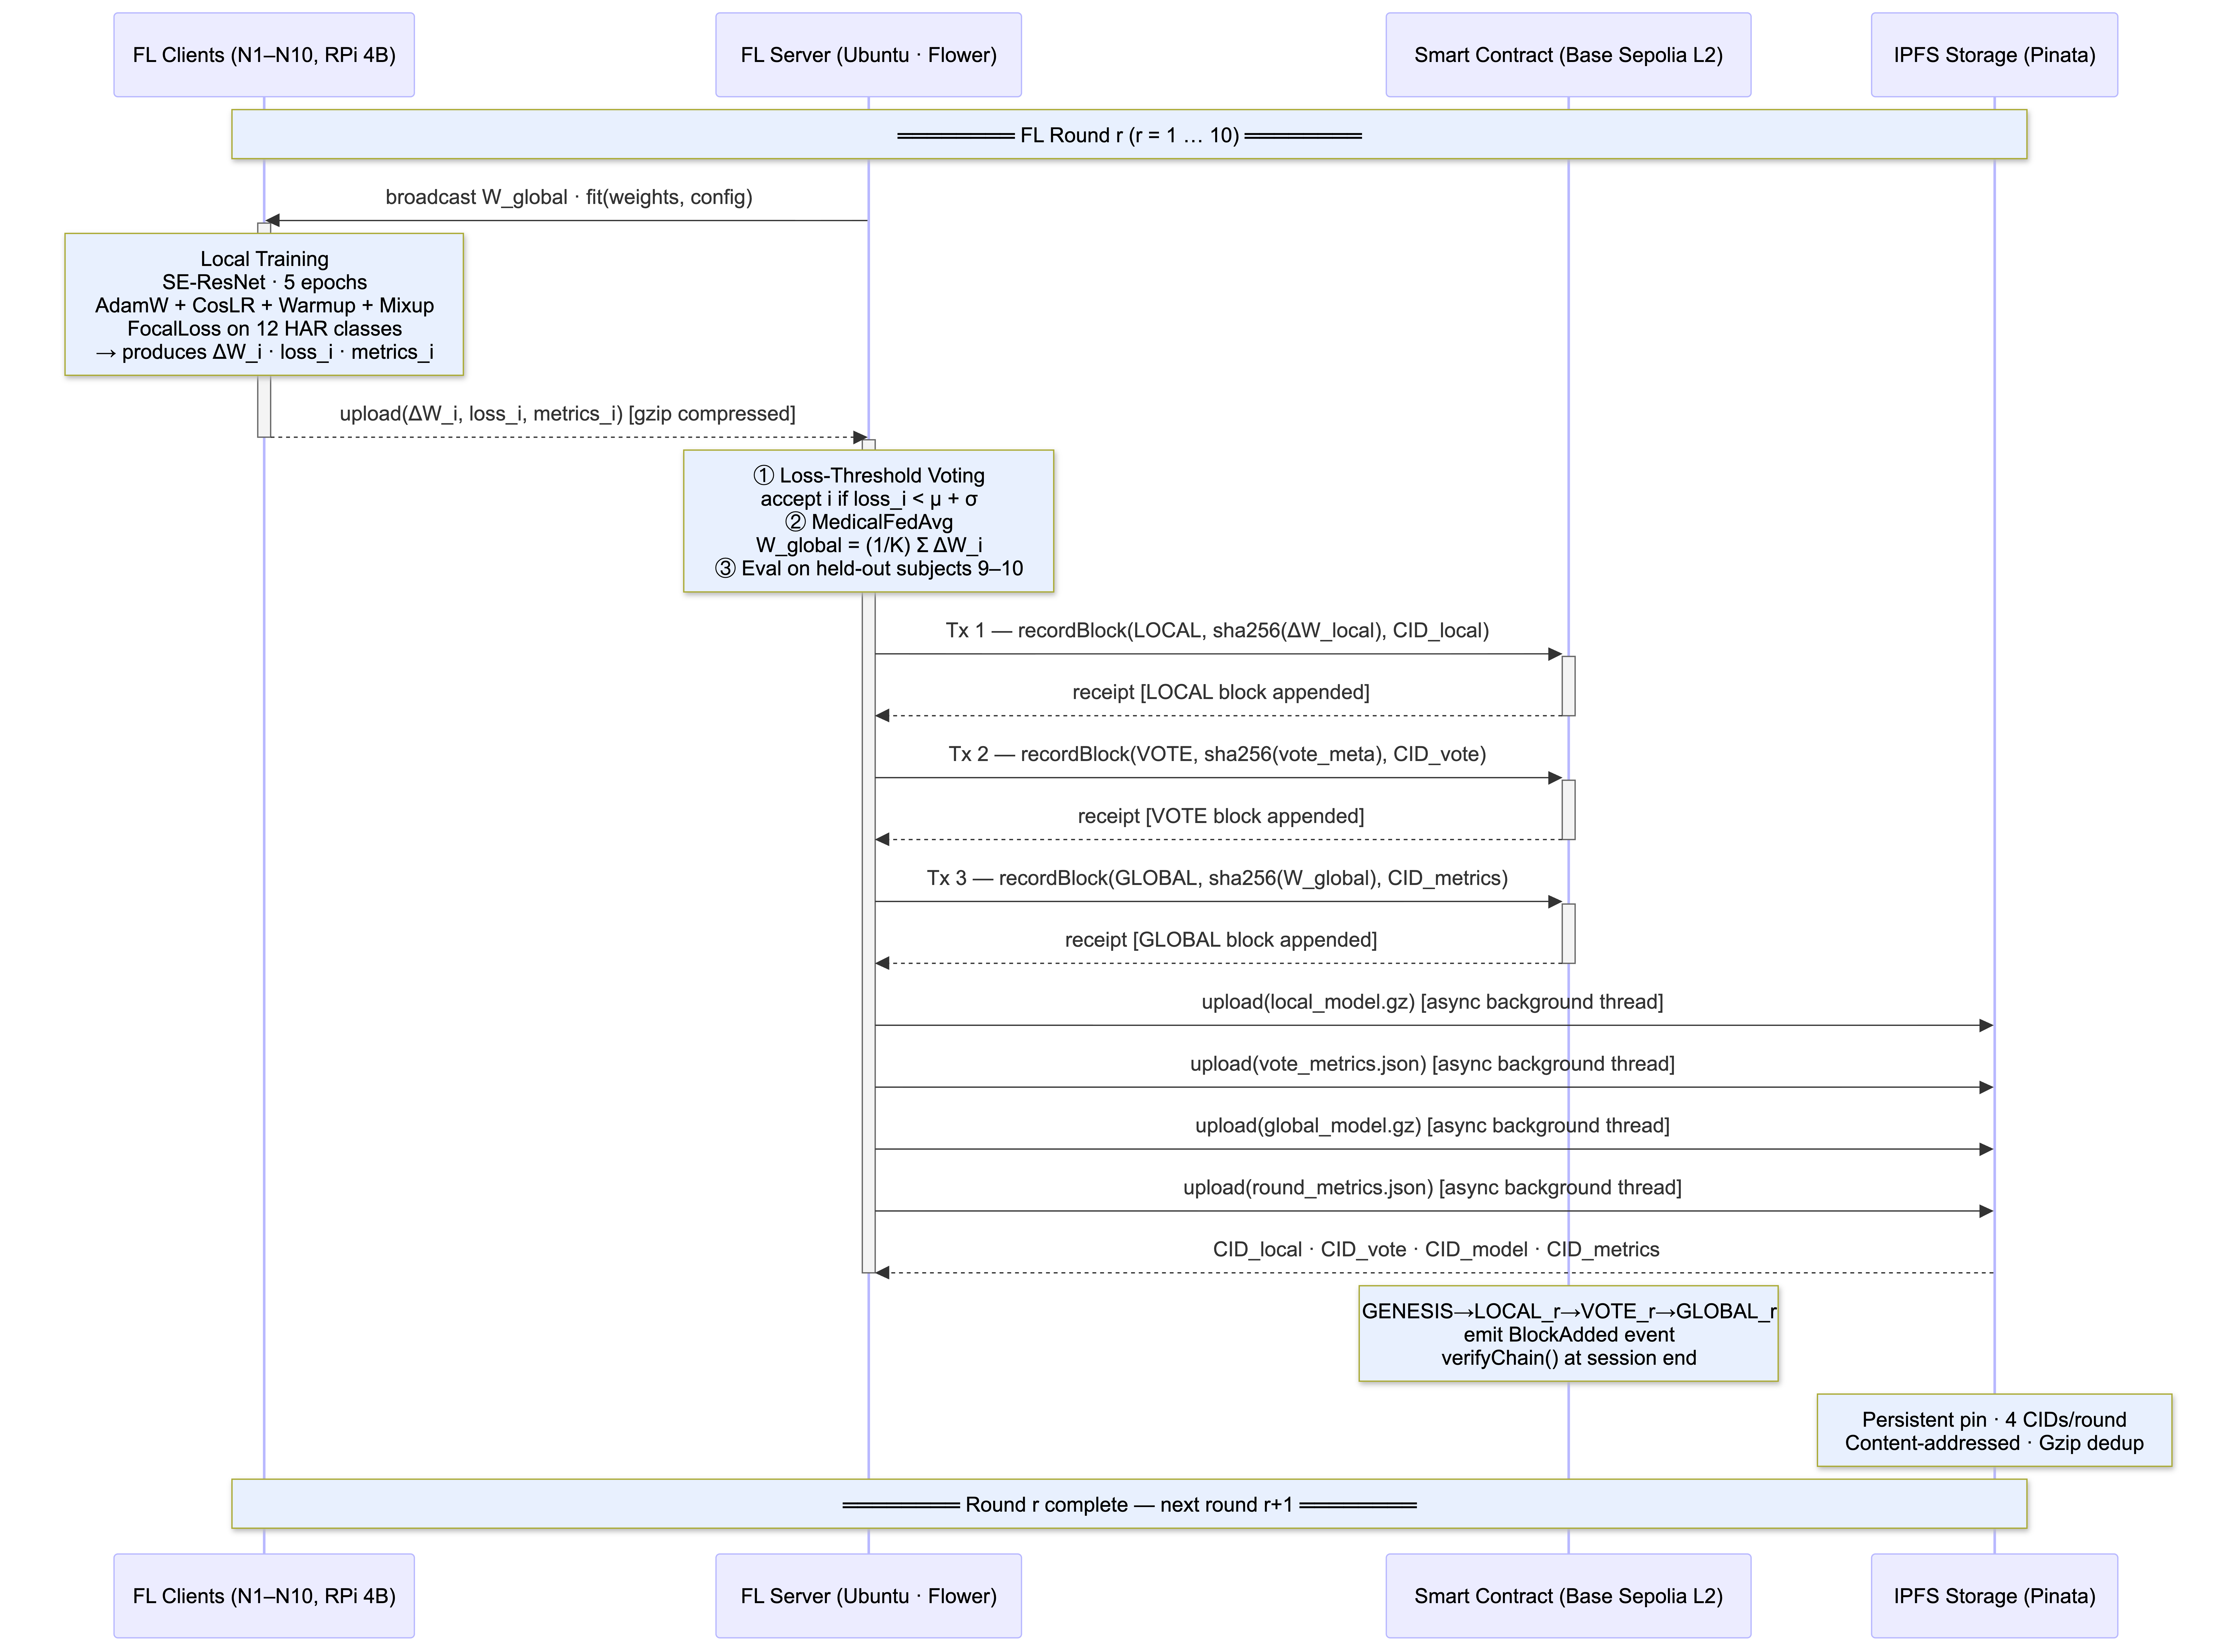
\includegraphics[width=0.95\textheight,keepaspectratio]{sequence_chart_02.png}
\caption{Round-level FLBL2 interaction sequence. The FL server coordinates
  model broadcast, client updates, loss-threshold voting, three on-chain write
  transactions (LOCAL/VOTE/GLOBAL), and asynchronous IPFS uploads, then closes
  the round and continues to $r{+}1$ with session-level chain verification.}
\label{fig:workflow}
\end{sidewaysfigure}

\begin{algorithm}[h]
\caption{Baseline per-round fire-and-wait blockchain write}
\label{alg:faw}
\begin{algorithmic}[1]
\Require Round $r$; artifacts $\mathit{cid}_{\mathrm{local}}, \mathit{cid}_{\mathrm{vote}}, \mathit{cid}_{\mathrm{global}}$
\State Upload $\mathit{cid}_{\mathrm{local}}, \mathit{cid}_{\mathrm{vote}}, \mathit{cid}_{\mathrm{global}}$ to IPFS (blocking, $\times$3 sequential)
\State $g_1 \leftarrow$ \texttt{eth\_estimateGas(recordLocal)} \quad; $g_2 \leftarrow$ \texttt{eth\_estimateGas(recordVote)} \quad; $g_3 \leftarrow$ \texttt{eth\_estimateGas(recordGlobal)}
\State $p \leftarrow$ \texttt{eth\_gasPrice} (called once per TX, $\times$3)
\State Send \texttt{recordLocal}$(\mathit{cid}_{\mathrm{local}})$ $\rightarrow h_1$ \quad;
       Send \texttt{recordVote}$(\mathit{cid}_{\mathrm{vote}})$ $\rightarrow h_2$ \quad;
       Send \texttt{recordGlobal}$(\mathit{cid}_{\mathrm{global}})$ $\rightarrow h_3$
\State \textbf{await} receipt of $h_1, h_2, h_3$ in parallel
\State Call \texttt{verifyChain()} \quad $\triangleright$ per-round integrity check
\end{algorithmic}
\end{algorithm}

\begin{algorithm}[h]
\caption{Optimized FL-Blockchain session protocol (FLBL2-OPT)}
\label{alg:opt}
\begin{algorithmic}[1]
\Require $S$\,=\,number of rounds per session
\State Start IPFS background upload thread
\State $\hat{g} \leftarrow$ \texttt{eth\_estimateGas} once for all TXs  \Comment{O1: cache}
\For{round $r = 1$ to $S$}
  \State Run local training on all clients (5 epochs each)
  \State MedicalFedAvg aggregation $\rightarrow w_r^{(g)}$
  \State Enqueue $(w_r^{(g)},\text{metrics}_r)$ to IPFS background thread  \Comment{O3: async}
  \State $\hat{p}_r \leftarrow$ \texttt{eth\_gasPrice} once for this round  \Comment{O2: cache}
  \State Send \texttt{recordLocal, recordVote, recordGlobal} using $\hat{g}, \hat{p}_r$ $\rightarrow h_1,h_2,h_3$
  \State \textbf{await} $h_1, h_2, h_3$ confirmed in parallel
\EndFor
\State \textbf{await} IPFS background thread completion  \Comment{O3: join}
\State Call \texttt{verifyChain()} once at session end  \Comment{O4: deferred}
\State Assert $\texttt{verifyChain()} = \texttt{true}$; log all CIDs and TX hashes
\end{algorithmic}
\end{algorithm}

The baseline protocol (Alg.~\ref{alg:faw}) issues $3N$ \texttt{eth\_estimateGas} and $3N$
\texttt{eth\_gasPrice} RPC calls per session---$O(N)$ network-bound operations in each
group---plus $3N$ blocking IPFS uploads on the round critical path.
Uploads dominate: the measured mean per-CID upload time is 11{,}436\,ms
(Table~\ref{tab:overhead}), giving an expected per-round IPFS blocking cost of
34{,}308\,ms, with a worst-case tail reaching $3\times190{,}830$\,ms under Pinata
congestion, which directly explains the $\sigma{=}67.3$\,s round-time standard
deviation observed across the ten baseline sessions.
Chain verification compounds the overhead further: at round $r$ the chain holds
$1{+}3r$ blocks, so each \texttt{verifyChain()} invocation performs $O(r)$ hash
comparisons; summed over $N$ rounds, the session-total verification work is
$\sum_{r=1}^{N}(1{+}3r)=N+\tfrac{3N(N+1)}{2}=O(N^2)$.
At $N{=}10$, a single session accumulates 175 block reads distributed across 10
calls on chains of 4, 7, 10, \ldots, 31 blocks respectively.
The baseline therefore carries an $O(N)$ critical-path IPFS penalty and an
$O(N^2)$ cumulative verification overhead per session.

FLBL2-OPT (Alg.~\ref{alg:opt}) eliminates the $O(N^2)$ verification term by
deferring \texttt{verifyChain()} to a single call at session end (O4): the scan
traverses $1{+}3N$ blocks exactly once, reducing the per-session verification cost
to $O(N)$.
Gas-limit estimation is pulled outside the training loop and computed once per
session (O1), cutting \texttt{eth\_estimateGas} calls from $3N$ to $O(1)$ and
recovering $\approx1{,}058$\,ms per round.
The gas price is fetched once per round instead of three times (O2), reducing
price-fetch calls from $3N$ to $N$ and recovering $\approx350$\,ms per round.
IPFS uploads are dispatched to a background thread (O3), reducing the per-round
critical-path upload term from $O(|A|)$---proportional to artifact size---to
$O(1)$ enqueue; the thread joins after the final round with no effect on the
aggregation or on-chain record structure.
The per-round critical path therefore reduces to $O(1)$ RPC calls, $O(1)$
transaction sends, and $O(1)$ enqueue, with confirmation latency set entirely
by the Base~L2 sequencer.
Concretely, O3 removes $\approx34{,}308$\,ms of mean blocking time per round from
the critical path and O1+O2+O4 contribute a further $\approx1{,}942$\,ms of
deterministic savings (Table~\ref{tab:opts}), together yielding the 22.4\% mean
round-time reduction and 57.6\% variance reduction reported in Table~\ref{tab:walltime}.

\FloatBarrier
% ============================================================
\section{Testbed Setup, Dataset, and Model}
\label{sec:impl}
This section presents the experimental foundation of the proposed FLBL2 framework by detailing the physical edge testbed, dataset, and model configuration used in this study. It describes the deployment of a multi-device ARM-based federated learning environment, the characteristics of the MHEALTH dataset, and the design of the lightweight deep learning model employed for human activity recognition. This section establishes the practical setup used to validate the proposed audit architecture under realistic edge computing conditions.

\subsection{Physical Testbed and Software Environment}

Ten Raspberry Pi~4 Model~B (4\,GB RAM, ARM Cortex-A72 at 1.5\,GHz) serve
as federated clients. All devices connect to the FL server over a shared
2.4\,GHz Wi-Fi access point using Ethernet-equivalent gRPC channels managed
by Flower SuperLink. The server runs the aggregation and blockchain middleware
on a Ubuntu workstation (Fig.~\ref{fig:testbed}). Table~\ref{tab:sw} lists
software versions. The entire stack---Flower framework, smart contract
tooling, and Pinata SDK---is deployed without modification from standard
package distributions, confirming that the FLBL2 design requires no
specialised infrastructure beyond a standard Python environment and an
Ethereum wallet with L2 funds.

\begin{figure}[htbp]
\centering
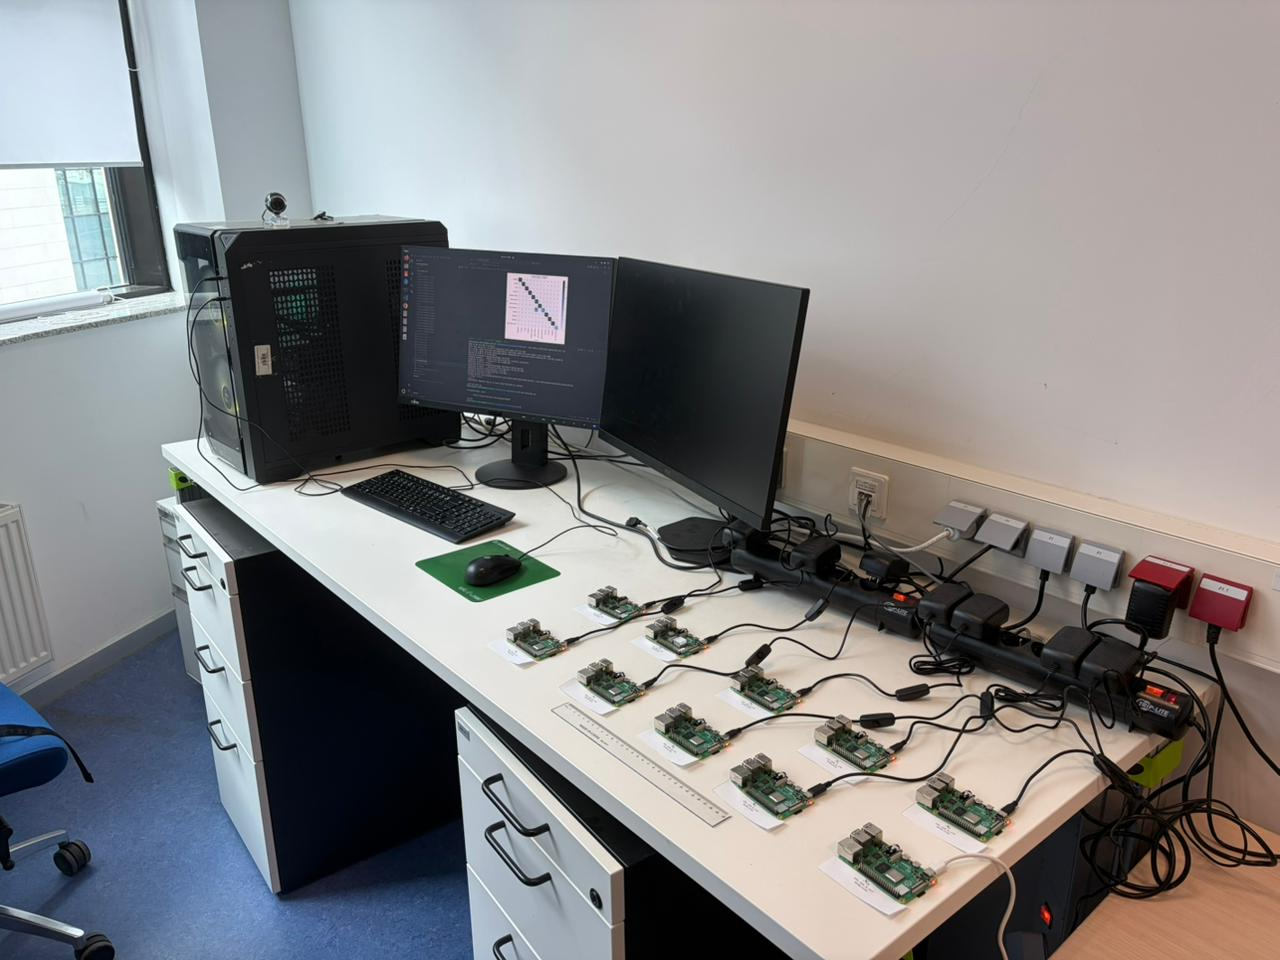
\includegraphics[width=0.88\linewidth]{10-nodes_with_Ubuntu_server_PC.jpeg}
\caption{Physical FLBL2 testbed: ten Raspberry Pi~4 Model B devices
  (N0--N9, foreground, each labelled) connected to the Ubuntu server
  workstation running Flower SuperLink and blockchain middleware
  (background, dual-monitor setup). The confusion matrix visible on the secondary monitor was captured live during the April~2026 experiment.
  The setup confirms ARM Cortex-A72 edge hardware running under sustained
  HAR training load for $>$9 hours without thermal throttling.}
\label{fig:testbed}
\end{figure}

\begin{table}[h]
\caption{Software stack.}
\label{tab:sw}
\centering\footnotesize
\begin{tabular}{ll}
\toprule
\textbf{Component} & \textbf{Version} \\
\midrule
Flower (flwr)        & 1.23 \\
PyTorch              & 2.3 \\
Python               & 3.11 \\
web3.py              & 7.x \\
Pinata SDK           & 3.x \\
Solidity compiler    & 0.8.20 \\
OS (RPi)             & Raspberry Pi OS Bookworm \\
\bottomrule
\end{tabular}
\end{table}

\subsection{MHEALTH Dataset, SE-ResNet Model, and Experiment Protocol}

The MHEALTH dataset~\cite{banos2014mhealth} contains inertial sensor
recordings from ten subjects performing 12 physical activities: standing,
sitting, lying, walking, climbing stairs, waist bending, frontal arm
elevation, knee bending, cycling, jogging, running, and jump front-back.
Sensors include a chest accelerometer, left-ankle accelerometer and
gyroscope, and right-arm accelerometer and gyroscope sampled at 50\,Hz.
Raw signals are segmented into 256-sample windows ($\approx$5.12\,s at 50\,Hz, 50\% overlap). The
subject-level non-IID partition follows the structure most commonly studied
in FL-HAR literature~\cite{aouedi2024harsurvey,shiri2025dlharsurvey}:
subjects~1--8 are assigned to the ten training devices (N0+N8 share subject~1,
N1+N9 share subject~2, and N2--N7 each hold one subject exclusively), while
subjects~9 and~10 form a fixed held-out global test set of 514 windows,
evaluated at the server after each aggregation.

The classifier is a Squeeze-and-Excitation ResNet~\cite{hu2018senet} adapted
for 1-D sensor input with approximately $920{,}000$ parameters and a
12-class output head. Training uses Focal Loss~\cite{lin2017focal}
($\gamma=2$) to address class imbalance, AdamW ($\text{lr}=0.002$,
$\text{wd}=10^{-4}$) with a cosine-annealing schedule, and Mixup augmentation
($\alpha=0.3$). Clients run $E=5$ local epochs per round with batch size~64.
The SE attention mechanism provides channel recalibration at negligible
parameter cost, which was found to improve convergence speed on the
subject-heterogeneous MHEALTH splits compared to standard ResNet.
Lightweight CNN architectures have shown strong results in comparable
e-health contexts~\cite{baltabay2023lightweight,yatbaz2021activity} and our
SE-ResNet design follows that principle.

We ran 20 independent sessions---10 \emph{Baseline} and 10 \emph{Optimized},
each comprising 10 aggregation rounds (100 rounds per variant, 200 total).
Sessions ran consecutively from 20:12 on 24~April~2026 to 05:31 on
25~April~2026. In the \emph{Baseline} variant, IPFS uploads block each round
synchronously, gas limits are estimated per transaction, gas prices are
fetched per transaction, and \texttt{verifyChain()} executes after each round.
The \emph{Optimized} variant applies four targeted changes: \textbf{O1}
caches the gas-limit estimate per round (1 RPC call instead of 3);
\textbf{O2} caches the gas price per round (1 fetch instead of 3);
\textbf{O3} moves IPFS uploads to a background thread so FL coordination
proceeds in parallel; \textbf{O4} defers \texttt{verifyChain()} to session
end rather than running it per round. These four changes are surgical---they
target the measured bottlenecks in the critical path while leaving the FL
logic, aggregation algorithm, and on-chain record structure completely
unchanged. Statistical comparisons use a two-sided Mann-Whitney~U test
(per-round wall times, $n_B = n_O = 100$) and a Wilcoxon signed-rank test
(final-round accuracy per session, $n=10$), both at $\alpha=0.05$.

{\sloppy\noindent%
The smart contract is deployed on Base mainnet (chain ID~8453) at
contract address
\texttt{0xBE3FeA\allowbreak C76293711\allowbreak C5D32426\allowbreak 860303Af\allowbreak E24cdf527}.
Full session logs, trained models, and per-round metrics are released
at \url{https://github.com/shinratttensei1/FLBL2}.\par}


\FloatBarrier
% ============================================================
\section{Experimental Results}
\label{sec:results}

The evaluation spans three observational tiers recorded for every round of
every session: \textit{server-level} global metrics produced after each
Flower aggregation step; \textit{device-level} per-client training and
evaluation telemetry logged directly on each RPi~4; and
\textit{infrastructure-level} blockchain and IPFS timing captured by the
middleware layer. Together, the 20 sessions ($10$ baseline + $10$ optimized,
each of 10 rounds) yield 220 global-metric records ($11$ rounds $\times$ 20
sessions), 2{,}000 device-training records (10 clients $\times$ 10 rounds
$\times$ 20 sessions), 2{,}000 client-evaluation records, 310 IPFS upload
timings from the baseline performance log, 310 transaction confirmation
records, and 840 on-chain pin-map entries.

\subsection{Federated Learning Quality: Convergence, Consistency, and Per-Class Performance}
\label{subsec:flquality}

Table~\ref{tab:metrics} enumerates every field collected at each observational tier;
this three-layer instrumentation enables end-to-end traceability from raw
device behavior through FL quality to on-chain audit state.

\begin{table}[t]
\caption{Three-tier metrics collected per round. All records are stored in
  \texttt{results.json} (NDJSON) per session; infrastructure timing comes
  from \texttt{perf\_*.log}.}
\label{tab:metrics}
\centering\footnotesize
\setlength{\tabcolsep}{3pt}
\begin{tabular}{llp{6.3cm}}
\toprule
\textbf{Tier} & \textbf{Granularity} & \textbf{Fields} \\
\midrule
Server / global & 1 record per round
  & accuracy, loss, macro-F1, weighted-F1, macro-precision,
    macro-recall, macro-specificity, macro-AUC,
    per-class F1/precision/recall/AUC (12 classes),
    confusion matrix, round wall time, blockchain block count,
    model payload bytes, IPFS CID list \\
\midrule
Device training & 10 records per round
  & client ID, train loss, training time (s), CPU\,\%,
    RAM (MB), CPU temperature (°C), \#examples, active classes \\
\midrule
Device evaluation & 10 records per round
  & client ID, eval accuracy, eval F1, eval AUC, eval loss,
    eval time (s), CPU\,\%, RAM (MB), CPU temperature (°C) \\
\midrule
Infrastructure & per round
  & IPFS upload time per CID (ms), gas-estimate RPC time (ms),
    gas-price fetch time (ms), TX send time (ms),
    TX confirmation time (ms), \texttt{verifyChain()} time (ms),
    total non-training overhead (ms) \\
\bottomrule
\end{tabular}
\end{table}

Table~\ref{tab:convergence} shows per-round mean accuracy and loss across
all ten sessions of each variant. Both variants converge along the same
trajectory: accuracy crosses 90\% by round~5, exceeds 95\% by round~7,
and stabilises above 96\% in rounds 9--10.

\begin{table}[t]
\caption{Per-round FL metrics (mean, $n=10$ sessions each).
  B\,=\,Baseline; O\,=\,Optimized.
  Accuracy columns also report $\pm$1\,std.}
\label{tab:convergence}
\centering\footnotesize
\setlength{\tabcolsep}{3.2pt}
\begin{tabular}{c cc cc cc cc}
\toprule
\multirow{2}{*}{\textbf{Rnd}} &
  \multicolumn{2}{c}{\textbf{Accuracy ($\pm$std)}} &
  \multicolumn{2}{c}{\textbf{Macro-F1}} &
  \multicolumn{2}{c}{\textbf{Macro-AUC}} &
  \multicolumn{2}{c}{\textbf{Loss}} \\
\cmidrule(lr){2-3}\cmidrule(lr){4-5}\cmidrule(lr){6-7}\cmidrule(lr){8-9}
& \textbf{B} & \textbf{O} & \textbf{B} & \textbf{O}
& \textbf{B} & \textbf{O} & \textbf{B} & \textbf{O} \\
\midrule
 0 & $0.097{\pm}0.051$ & $0.084{\pm}0.046$ & 0.025 & 0.021 & 0.517 & 0.523 & 2.487 & 2.484 \\
 1 & $0.296{\pm}0.073$ & $0.232{\pm}0.077$ & 0.215 & 0.159 & 0.896 & 0.885 & 2.302 & 2.301 \\
 2 & $0.596{\pm}0.072$ & $0.617{\pm}0.049$ & 0.532 & 0.560 & 0.962 & 0.966 & 1.493 & 1.494 \\
 3 & $0.781{\pm}0.056$ & $0.797{\pm}0.045$ & 0.763 & 0.775 & 0.988 & 0.979 & 1.073 & 1.079 \\
 4 & $0.890{\pm}0.029$ & $0.884{\pm}0.038$ & 0.884 & 0.880 & 0.985 & 0.993 & 0.694 & 0.680 \\
 5 & $0.921{\pm}0.047$ & $0.936{\pm}0.050$ & 0.916 & 0.933 & 0.995 & 0.990 & 0.474 & 0.523 \\
 6 & $0.961{\pm}0.020$ & $0.927{\pm}0.037$ & 0.961 & 0.924 & 0.999 & 0.996 & 0.312 & 0.394 \\
 7 & $0.963{\pm}0.027$ & $0.952{\pm}0.019$ & 0.962 & 0.950 & 1.000 & 0.996 & 0.287 & 0.343 \\
 8 & $0.947{\pm}0.039$ & $0.948{\pm}0.029$ & 0.946 & 0.948 & 1.000 & 0.997 & 0.265 & 0.293 \\
 9 & $0.970{\pm}0.031$ & $0.955{\pm}0.029$ & 0.969 & 0.954 & 1.000 & 0.998 & 0.225 & 0.270 \\
10 & $0.962{\pm}0.029$ & $0.957{\pm}0.026$ & 0.961 & 0.956 & 0.999 & 0.997 & 0.203 & 0.248 \\
\bottomrule
\end{tabular}
\end{table}

A Wilcoxon signed-rank test on final-round accuracy yields $p=0.103$,
confirming that the two variants produce statistically equivalent FL quality.
The blockchain middleware changes affect round timing only, not model
convergence. Both variants achieve macro-AUC $\geq0.995$ from round~5
onward, demonstrating strong class separation across all 12 activities.
Precision ($\geq0.972$) and specificity ($\geq0.996$) at round~10 indicate
very few false positives, critical for wearable activity recognition.

Figure~\ref{fig:convergence} visualises both mean accuracy and mean macro-F1
across all 11 rounds, giving a clearer view of quality convergence and metric
consistency between baseline and optimized variants.

\begin{figure}[htbp]
\centering
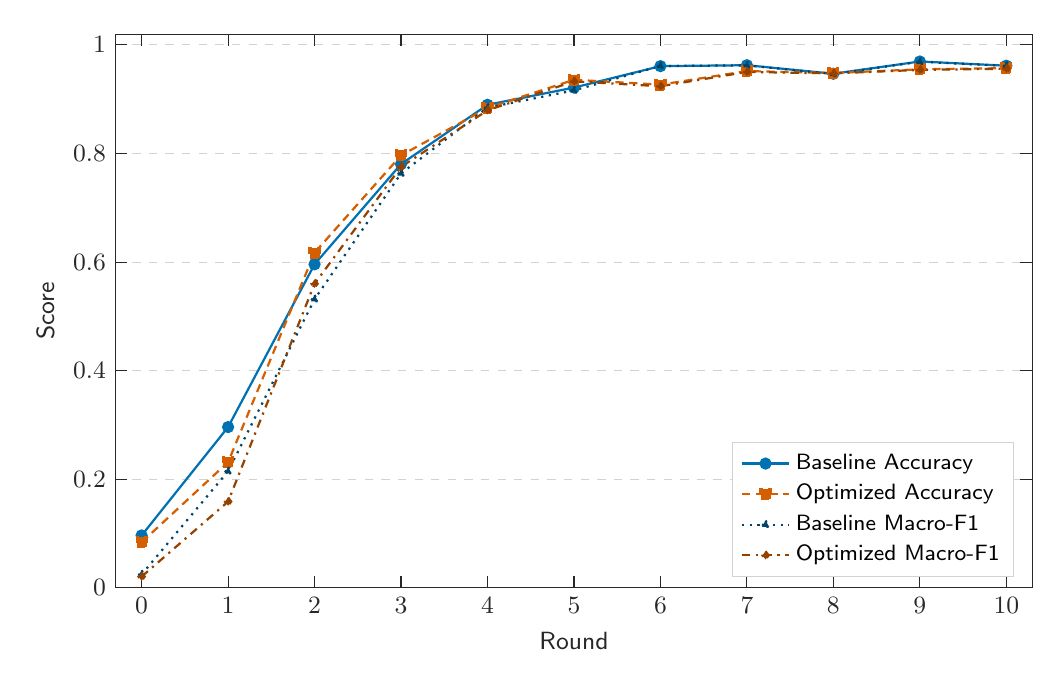
\begin{tikzpicture}
\begin{axis}[
  width=0.96\linewidth, height=0.58\linewidth,
  scale only axis,
  axis line style={clrAxis,thin},
  tick style={clrAxis,thin},
  ticklabel style={font=\small\sffamily,color=clrAxis},
  label style={font=\small\sffamily,color=clrAxis},
  ymajorgrids=true,
  grid style={clrGrid,thin,dashed},
  xlabel={Round},
  ylabel={Score},
  xtick={0,1,...,10},
  ytick={0,0.2,0.4,0.6,0.8,1.0},
  ymin=0, ymax=1.02,
  xmin=-0.3, xmax=10.3,
  legend style={font=\footnotesize\sffamily,draw=clrGrid,fill=white,
    at={(0.98,0.02)},anchor=south east},
  legend cell align=left,
]
\addplot[color=clrAcc, thick, mark=*, mark size=1.8pt] coordinates {
  (0,0.0965)(1,0.2961)(2,0.5959)(3,0.7805)(4,0.8897)
  (5,0.9214)(6,0.9609)(7,0.9626)(8,0.9469)(9,0.9695)(10,0.9617)
};
\addlegendentry{Baseline Accuracy}

\addplot[color=clrLoss, thick, mark=square*, mark size=1.8pt,
         densely dashed] coordinates {
  (0,0.0839)(1,0.2315)(2,0.6173)(3,0.7965)(4,0.8839)
  (5,0.9358)(6,0.9268)(7,0.9518)(8,0.9482)(9,0.9551)(10,0.9572)
};
\addlegendentry{Optimized Accuracy}

\addplot[color=clrAcc!60!black, thick, dotted,
         mark=triangle*, mark size=1.5pt] coordinates {
  (0,0.0246)(1,0.2147)(2,0.5316)(3,0.7632)(4,0.8843)
  (5,0.9162)(6,0.9612)(7,0.9623)(8,0.9464)(9,0.9690)(10,0.9614)
};
\addlegendentry{Baseline Macro-F1}

\addplot[color=clrLoss!70!black, thick, dashdotted,
         mark=diamond*, mark size=1.5pt] coordinates {
  (0,0.0206)(1,0.1588)(2,0.5601)(3,0.7754)(4,0.8795)
  (5,0.9329)(6,0.9239)(7,0.9502)(8,0.9476)(9,0.9540)(10,0.9561)
};
\addlegendentry{Optimized Macro-F1}
\end{axis}
\end{tikzpicture}
\caption{Round-wise convergence trends from all 20 sessions (10 baseline,
  10 optimized). Solid lines show mean accuracy and patterned lines show
  mean macro-F1. Both variants follow near-identical quality trajectories,
  consistent with the Wilcoxon result ($p=0.103$).}
\label{fig:convergence}
\end{figure}

Across sessions, baseline peak accuracy is $0.986\pm0.016$ (macro-AUC
$1.000\pm0.000$, macro-F1 $0.986\pm0.016$). The optimized variant
reaches $0.972\pm0.021$. One session (\texttt{baseline\_20260425\_012342},
round~8) achieved accuracy~$=1.000$ with all 12 per-class F1 scores equal
to 1.000 on the 514-window test set.

Table~\ref{tab:sessions} shows per-session final-round accuracy, peak
accuracy, and mean round wall time for all 20 sessions. The baseline
outlier (\texttt{221512}, wall\,=\,200.9\,s) is caused by two consecutive
IPFS upload spikes ($>150$\,s each) in rounds 5 and 6. The optimized
sessions are uniformly under 95\,s, with only one exception (session
\texttt{000013}: R9 confirmation delay of 226\,s).

\begin{table}[t]
\caption{Per-session R10 accuracy, peak accuracy, and mean round wall
  time. B\,=\,Baseline; O\,=\,Optimized.}
\label{tab:sessions}
\centering\footnotesize
\setlength{\tabcolsep}{4pt}
\begin{tabular}{llccc}
\toprule
\textbf{Session} & \textbf{V.} & \textbf{R10 Acc} & \textbf{Peak Acc} & \textbf{Mean Wall (s)} \\
\midrule
20260424\_201227 & B & 0.9339 & 0.9728 & \phantom{0}88.4 \\
20260424\_210558 & B & 0.9922 & 1.0000 & 145.3 \\
20260424\_221512 & B & 0.9202 & 0.9650 & 200.9$^{\dagger}$ \\
20260424\_233404 & B & 0.9728 & 0.9903 & \phantom{0}74.1 \\
20260425\_003015 & B & 0.9572 & 0.9883 & \phantom{0}79.8 \\
20260425\_012342 & B & 0.9942 & \textbf{1.0000} & \phantom{0}83.1 \\
20260425\_022158 & B & 0.9553 & 0.9981 & \phantom{0}66.0 \\
20260425\_031417 & B & 0.9903 & 0.9942 & \phantom{0}79.7 \\
20260425\_040906 & B & 0.9825 & 0.9961 & \phantom{0}65.9 \\
20260425\_050237 & B & 0.9183 & 0.9572 & \phantom{0}76.4 \\
\midrule
20260424\_204043 & O & 0.9805 & 0.9805 & \phantom{0}75.0 \\
20260424\_214450 & O & 0.9767 & \textbf{1.0000} & \phantom{0}93.4 \\
20260424\_230422 & O & 0.9864 & 0.9864 & \phantom{0}80.9 \\
20260425\_000013 & O & 0.9125 & 0.9280 & \phantom{0}85.2 \\
20260425\_005637 & O & 0.9572 & 0.9611 & \phantom{0}72.5 \\
20260425\_015329 & O & 0.9553 & 0.9591 & \phantom{0}77.8 \\
20260425\_025021 & O & 0.9689 & 0.9903 & \phantom{0}62.8 \\
20260425\_034413 & O & 0.9125 & 0.9572 & \phantom{0}67.7 \\
20260425\_043806 & O & 0.9572 & 0.9805 & \phantom{0}67.6 \\
20260425\_053117 & O & 0.9650 & 0.9747 & \phantom{0}62.2 \\
\midrule
\multicolumn{2}{l}{\textbf{Baseline mean}} & $0.962{\pm}0.029$ & $0.986{\pm}0.016$ & $\mathbf{96.0{\pm}67.3}$ \\
\multicolumn{2}{l}{\textbf{Optimized mean}} & $0.957{\pm}0.026$ & $0.972{\pm}0.021$ & $\mathbf{74.5{\pm}28.5}$ \\
\bottomrule
\multicolumn{5}{l}{$^{\dagger}$Outlier caused by two consecutive IPFS upload spikes.}
\end{tabular}
\end{table}

Table~\ref{tab:perclass} breaks down R10 F1 and AUC by activity class
(mean over 10 sessions each). Eight of twelve activities achieve
F1\,$\geq\!0.99$ in both variants, confirming that the federated model
generalises strongly. The three hardest activities---\textit{Sitting},
\textit{Waist Bends Forward}, and \textit{Knees Bending}---show greater
variance across sessions (std up to 0.161) because these quasi-static
postures share overlapping inertial signatures in the MHEALTH dataset.
Jump Front and Back (only 16 test windows) reaches F1\,$=$\,1.000
in every session of both variants.

\begin{table}[t]
\caption{Per-class F1 and AUC at round 10 (mean $\pm$ std, $n=10$).
  Std shown only where $>0$.}
\label{tab:perclass}
\centering\footnotesize
\setlength{\tabcolsep}{3.5pt}
\begin{tabular}{lcccc}
\toprule
\textbf{Activity} &
  \textbf{B-F1} & \textbf{B-AUC} &
  \textbf{O-F1} & \textbf{O-AUC} \\
\midrule
Standing        & $1.000$            & 1.000 & $1.000$            & 1.000 \\
Sitting         & $0.876{\pm}0.161$  & 0.991 & $0.933{\pm}0.141$  & 0.999 \\
Lying           & $1.000$            & 1.000 & $1.000$            & 1.000 \\
Walking         & $1.000$            & 1.000 & $1.000$            & 1.000 \\
Climbing Stairs & $0.993{\pm}0.015$  & 1.000 & $1.000$            & 1.000 \\
Waist Bends Fwd & $0.895{\pm}0.078$  & 1.000 & $0.829{\pm}0.050$  & 1.000 \\
Front Arm Elev. & $0.921{\pm}0.102$  & 1.000 & $0.959{\pm}0.087$  & 1.000 \\
Knees Bending   & $0.854{\pm}0.114$  & 0.998 & $0.757{\pm}0.094$  & 0.960 \\
Cycling         & $1.000$            & 1.000 & $1.000$            & 1.000 \\
Jogging         & $0.999{\pm}0.003$  & 1.000 & $0.998{\pm}0.005$  & 1.000 \\
Running         & $0.999{\pm}0.003$  & 1.000 & $0.998{\pm}0.005$  & 1.000 \\
Jump Front+Back & $1.000$            & 1.000 & $1.000$            & 1.000 \\
\midrule
\textbf{Macro}  & $\mathbf{0.962{\pm}0.029}$ & \textbf{0.999} &
                  $\mathbf{0.957{\pm}0.026}$ & \textbf{0.997} \\
\bottomrule
\end{tabular}
\end{table}

Figure~\ref{fig:perclass} plots per-class F1 for both variants as a bar
chart, making the four difficult classes immediately visible.
Figure~\ref{fig:cm_comparison} shows the round-10 confusion matrices for
the best session of each variant.

\begin{figure}[htbp]
\centering
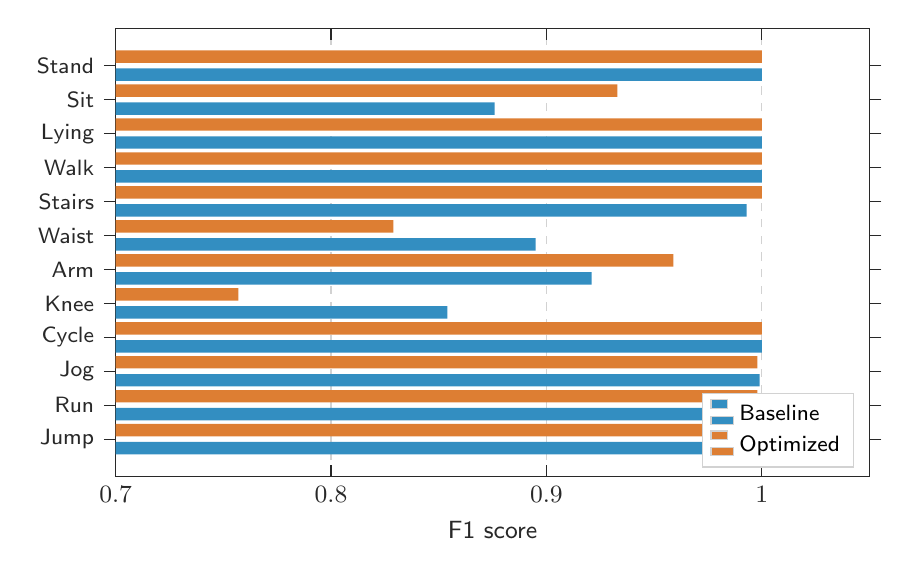
\begin{tikzpicture}
\begin{axis}[
  width=0.92\linewidth, height=0.60\linewidth,
  xbar,
  bar width=4.5pt,
  xlabel={F1 score},
  symbolic y coords={
    Jump,Run,Jog,Cycle,Knee,Arm,Waist,Stairs,Walk,Lying,Sit,Stand},
  ytick=data,
  yticklabel style={font=\footnotesize\sffamily},
  xmin=0.70, xmax=1.05,
  xtick={0.70,0.80,0.90,1.00},
  axis line style={clrAxis,thin},
  tick style={clrAxis,thin},
  ticklabel style={font=\small\sffamily,color=clrAxis},
  label style={font=\small\sffamily,color=clrAxis},
  xmajorgrids=true,
  grid style={clrGrid,thin,dashed},
  legend style={font=\footnotesize\sffamily,at={(0.98,0.02)},
    anchor=south east,draw=clrGrid,fill=white},
  legend cell align=left,
]
\addplot[xbar,fill=clrAcc!80,draw=none] coordinates {
  (1.000,Stand)(0.876,Sit)(1.000,Lying)(1.000,Walk)
  (0.993,Stairs)(0.895,Waist)(0.921,Arm)(0.854,Knee)
  (1.000,Cycle)(0.999,Jog)(0.999,Run)(1.000,Jump)
};
\addlegendentry{Baseline}
\addplot[xbar,fill=clrLoss!80,draw=none] coordinates {
  (1.000,Stand)(0.933,Sit)(1.000,Lying)(1.000,Walk)
  (1.000,Stairs)(0.829,Waist)(0.959,Arm)(0.757,Knee)
  (1.000,Cycle)(0.998,Jog)(0.998,Run)(1.000,Jump)
};
\addlegendentry{Optimized}
\end{axis}
\end{tikzpicture}
\caption{Per-class F1 at round~10 (mean across 10 sessions each).
  Difficult quasi-static activities (Sitting, Waist Bends, Knees Bending)
  show lower F1 and higher inter-session variance.}
\label{fig:perclass}
\end{figure}

\begin{figure}[htbp]
\centering
\begin{minipage}[t]{0.48\linewidth}
  \centering
  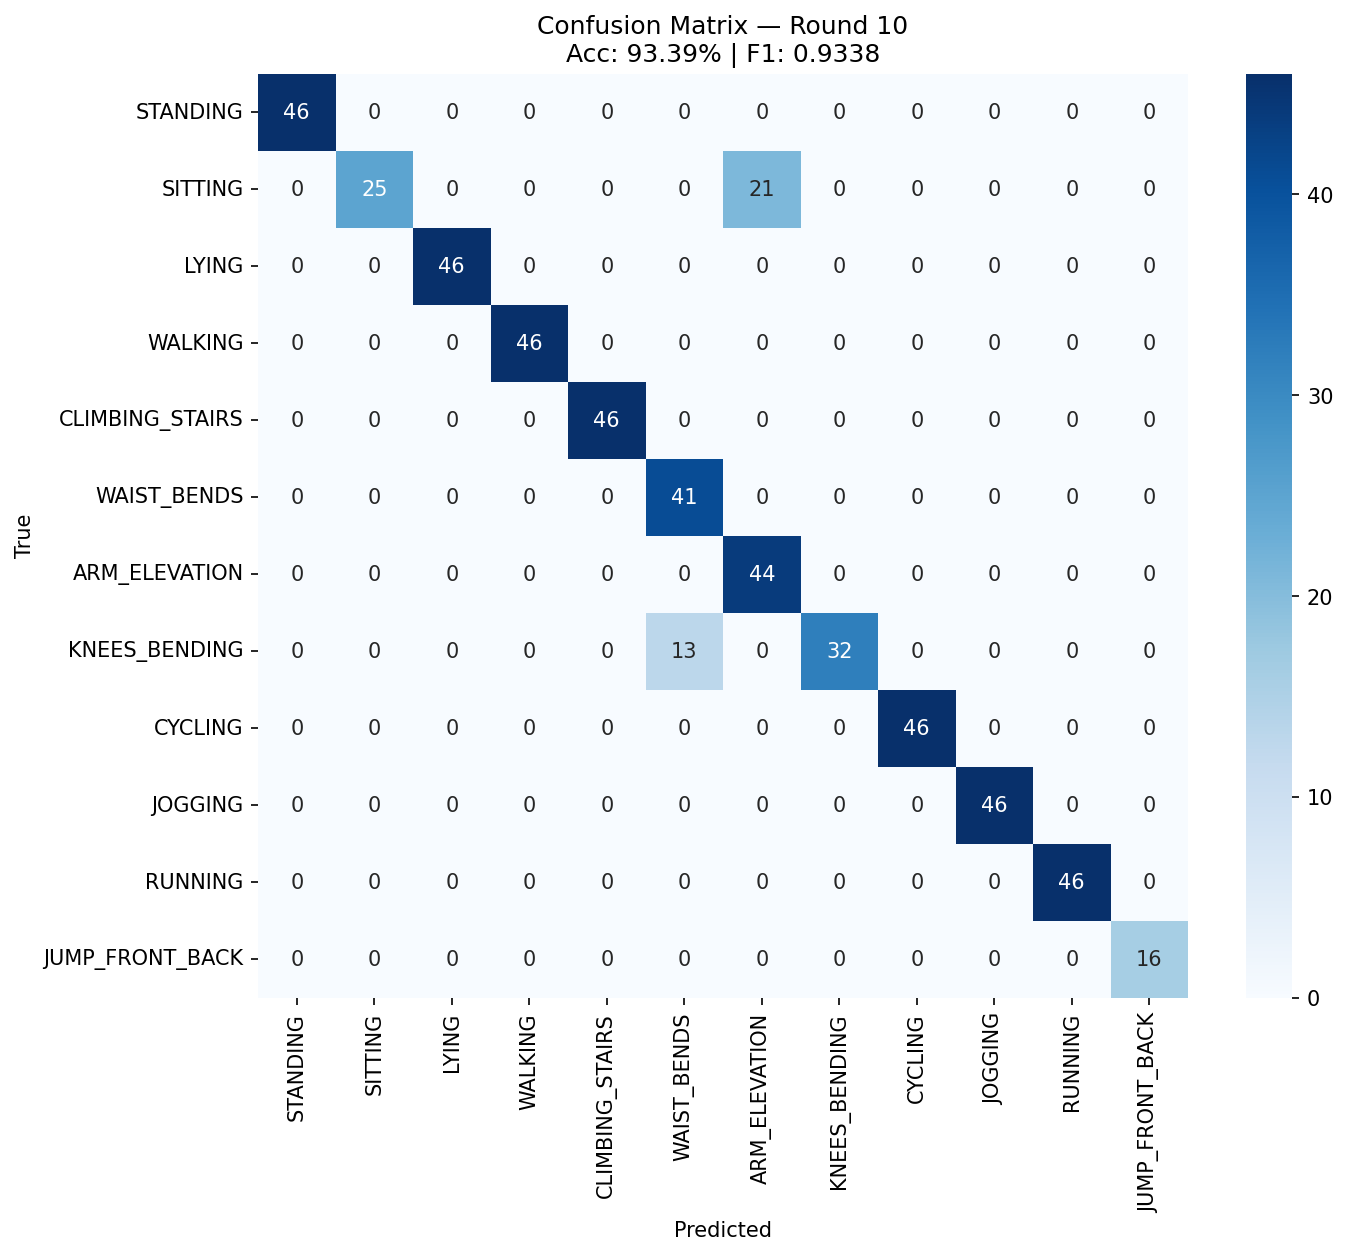
\includegraphics[width=\linewidth]{cm_baseline_r10.png}
\end{minipage}\hfill
\begin{minipage}[t]{0.48\linewidth}
  \centering
  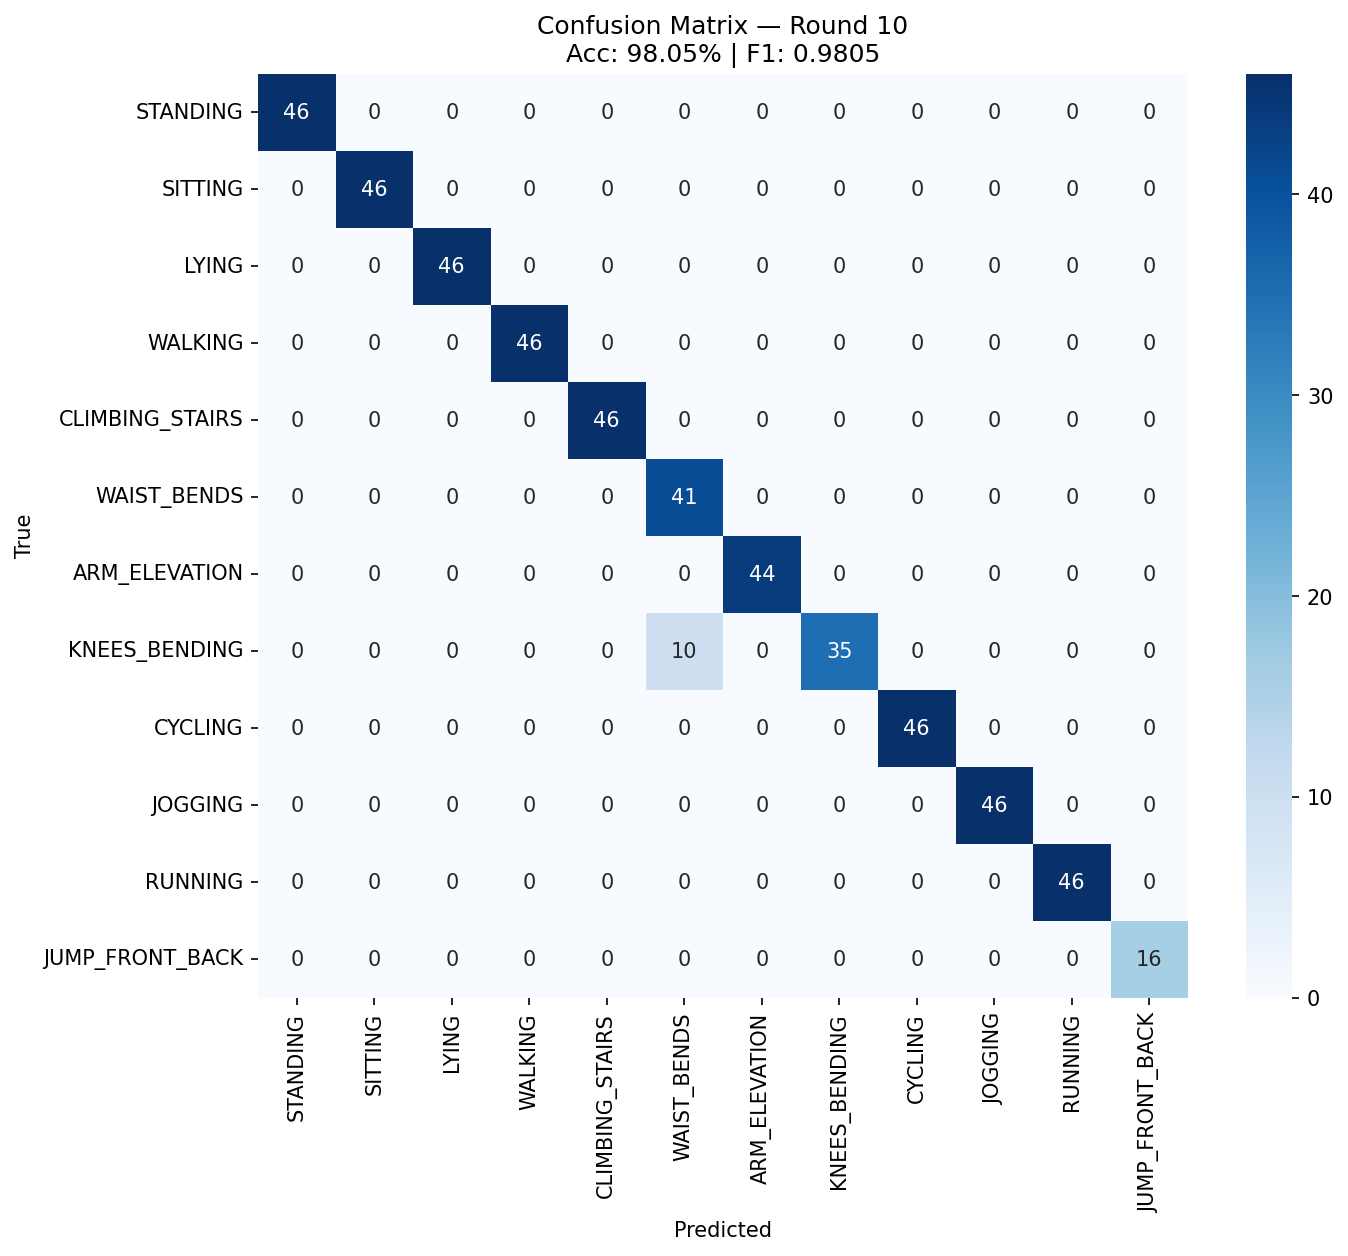
\includegraphics[width=\linewidth]{cm_optimized_r10.png}
\end{minipage}
\caption{Confusion matrices at round~10. \emph{Left}: best baseline session
  (\texttt{baseline\_20260425\_012342}, Acc\,=\,99.42\%, macro-F1\,=\,0.9942).
  \emph{Right}: best optimized session
  (\texttt{optimized\_20260424\_204043}, Acc\,=\,98.05\%, macro-F1\,=\,0.9805).
  In both variants the principal off-diagonal mass is Knees~Bending
  mislabelled as Waist~Bends (3 and 10 errors respectively), reflecting
  the similar pelvis-region inertial signatures of these quasi-static
  postures. All locomotion and cycling classes are classified perfectly.}
\label{fig:cm_comparison}
\end{figure}

\subsection{Per-Device Hardware Behavior}
\label{subsec:hw}

Table~\ref{tab:hw} reports per-client training and evaluation
statistics aggregated over all 100 training rounds (10 rounds $\times$
10 baseline sessions) per device. Clients are grouped by observed
training time: Group~A (N0, N1, N2, N4, N9) averages $17.94\pm0.12$\,s
and Group~B (N3, N5, N6, N7, N8) averages $19.15\pm0.13$\,s. The 6.7\%
time difference is consistent and likely reflects kernel scheduling
differences related to subject-specific data volume per device.

\begin{table}[t]
\caption{Per-client training and evaluation telemetry (baseline, $n=100$ rounds each).
  Gr\,=\,speed group; TrainT\,=\,mean training time (s);
  Temp\,=\,mean/max temperature (°C); EvalT\,=\,mean evaluation time (s).}
\label{tab:hw}
\centering\footnotesize
\setlength{\tabcolsep}{3pt}
\begin{tabular}{cccrrrrrr}
\toprule
\textbf{Cl.} & \textbf{Gr.} & \textbf{TrainT} & \textbf{CPU\%}
  & \textbf{RAM} & \textbf{Temp (mean/max)} & \textbf{EvalT} \\
\midrule
N0 & A & $17.97{\pm}0.11$ & 83.3 & 1069 & 69.2\,/\,74.0 & 2.083 \\
N1 & A & $17.93{\pm}0.12$ & 83.3 & 1071 & 62.6\,/\,66.2 & 2.095 \\
N2 & A & $17.94{\pm}0.13$ & 83.2 & 1067 & 64.1\,/\,69.1 & 2.089 \\
N3 & B & $19.16{\pm}0.12$ & 83.5 & 1037 & 61.0\,/\,65.7 & 2.121 \\
N4 & A & $17.96{\pm}0.13$ & 83.3 & 1069 & 67.7\,/\,71.1 & 2.097 \\
N5 & B & $19.15{\pm}0.12$ & 83.5 & 1039 & 63.5\,/\,66.7 & 2.185 \\
N6 & B & $19.14{\pm}0.17$ & 83.4 & 1042 & 61.8\,/\,65.7 & 2.141 \\
N7 & B & $19.16{\pm}0.14$ & 83.5 & 1041 & 62.5\,/\,66.2 & 2.115 \\
N8 & B & $19.16{\pm}0.13$ & 83.5 & 1060 & 61.4\,/\,65.2 & 2.115 \\
N9 & A & $17.91{\pm}0.12$ & 83.2 & \phantom{0}979 & 61.4\,/\,65.2 & 2.058 \\
\midrule
\textbf{All} & -- & $18.55{\pm}0.62$ & 83.4 & 1047 & 63.7\,/\,74.0 & 2.110 \\
\bottomrule
\end{tabular}
\end{table}

Client~C0 is a persistent thermal outlier: its mean temperature is
6.6°C above the fleet mean and it reaches 74.0°C, the closest to the
ARM Cortex-A72 throttle threshold of 80°C across the entire experiment.
Client C9 consistently uses the least RAM (979\,MB vs.\ 1047\,MB fleet
mean), reflecting its smaller data partition (subject~2 alone). CPU
utilisation is 83.4\% across all 2{,}000 device-round observations and
both variants, confirming that local training saturates device compute
independently of blockchain configuration. Evaluation on 514 windows
takes only 2.11\,s per device.

\subsection{Blockchain Middleware: Baseline Characterization and Four Optimizations}
\label{subsec:opts}

Table~\ref{tab:overhead} decomposes the per-round middleware overhead
measured from 310 baseline rounds. IPFS uploads and transaction
confirmations are the two dominant costs, but they exhibit fundamentally
different statistical behavior: confirmation time is determined by the
Base~L2 sequencer (external) and confirms predictably in tens of seconds;
IPFS upload time is driven by Pinata~Cloud network conditions and has a
mean-to-max ratio of $1{:}16.7$, making it the root cause of baseline
round-time tail latency.

\begin{table}[t]
\caption{Middleware overhead per component in the baseline variant
  ($n=310$ rounds). Gas estimation and price fetch are 3 calls/round;
  TX send and confirmation are 3 per round (parallelised for confirmation).}
\label{tab:overhead}
\centering\scriptsize
\setlength{\tabcolsep}{2pt}
\begin{tabular}{lrrrr}
\toprule
\textbf{Component} & \textbf{Mean (ms)} & \textbf{Std (ms)}
  & \textbf{Min (ms)} & \textbf{Max (ms)} \\
\midrule
IPFS upload (per CID, $\times$3/rnd)
  & 11{,}436 & 30{,}621 & \phantom{0}647 & 190{,}830 \\
Gas estimation (\texttt{estimateGas})
  & \phantom{0}529 & \phantom{00}253 & \phantom{0}284 & \phantom{00}2{,}377 \\
Gas price fetch (\texttt{gasPrice})
  & \phantom{0}175 & \phantom{00}102 & \phantom{00}93 & \phantom{00,0}921 \\
TX send                                
  & \phantom{0}336 & \phantom{00}162 & \phantom{0}199 & \phantom{00}1{,}531 \\
\texttt{verifyChain()} (per round)     
  & \phantom{0}534 & \phantom{00}237 & \phantom{0}306 & \phantom{00}1{,}843 \\
TX confirmation (per round, max of 3)  
  & 58{,}533 & 68{,}568 & \phantom{00}103 & 416{,}165 \\
\midrule
\textbf{Non-confirm overhead (per round)}
  & \textbf{38{,}000} & -- & -- & -- \\
\textbf{Total overhead incl.\ confirm}
  & \textbf{96{,}500} & -- & -- & -- \\
\bottomrule
\end{tabular}
\end{table}

Three IPFS uploads per round compound the upload variance: the expected
blocking time is $3{\times}11{,}436{=}34{,}308$\,ms but can reach
$3{\times}190{,}830{=}572{,}490$\,ms in the worst case, far exceeding any
confirmation delay. In round~5 of session \texttt{221512}, two uploads
exceeded 150\,s each, producing a single-round wall time of 421.7\,s.
Round-level overhead excluding confirmation is $1{,}820\pm740$\,ms
(gas estimation + gas price + TX send + verifyChain), confirming that
non-IPFS, non-confirmation components are fast and predictable.

Figure~\ref{fig:txpin_raw} summarizes blockchain and IPFS outcome counts
per variant. Table~\ref{tab:opts} quantifies the contribution of each optimization
to per-round latency reduction.

\begin{figure}[htbp]
\centering
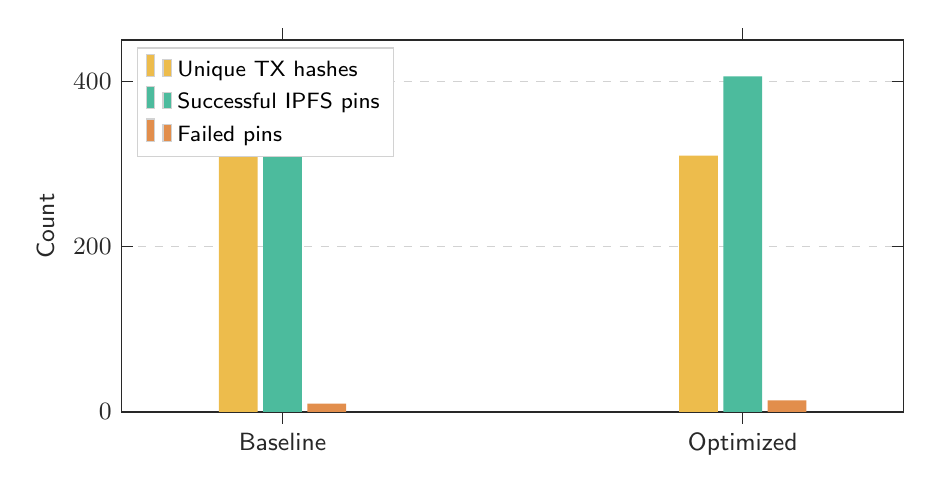
\begin{tikzpicture}
\begin{axis}[
  width=0.95\linewidth, height=0.52\linewidth,
  ybar,
  bar width=14pt,
  ymin=0, ymax=450,
  ylabel={Count},
  symbolic x coords={Baseline,Optimized},
  xtick=data,
  enlarge x limits=0.35,
  axis line style={clrAxis,thin},
  tick style={clrAxis,thin},
  ticklabel style={font=\small\sffamily,color=clrAxis},
  label style={font=\small\sffamily,color=clrAxis},
  ymajorgrids=true,
  grid style={clrGrid,thin,dashed},
  legend style={font=\footnotesize\sffamily,draw=clrGrid,fill=white,
    at={(0.02,0.98)},anchor=north west},
  legend cell align=left,
]
\addplot[fill=clrChain!70, draw=none] coordinates {(Baseline,310) (Optimized,310)};
\addlegendentry{Unique TX hashes}
\addplot[fill=clrIPFS!70, draw=none] coordinates {(Baseline,410) (Optimized,406)};
\addlegendentry{Successful IPFS pins}
\addplot[fill=clrAgg!70, draw=none] coordinates {(Baseline,10) (Optimized,14)};
\addlegendentry{Failed pins}
\end{axis}
\end{tikzpicture}
\caption{Raw blockchain/IPFS outcomes parsed from
  \texttt{outputs/tx\_pin\_map.csv}. Both variants produce the same number
  of unique on-chain transactions (310), while pin failures remain low
  (10 baseline, 14 optimized) over 420 pins per variant.}
\label{fig:txpin_raw}
\end{figure}

\begin{table}[t]
\caption{Per-round latency savings from each optimization.
  Savings are computed from baseline per-call measurements
  ($n=310$) and the changed call frequency in the optimized variant.}
\label{tab:opts}
\centering\footnotesize
\setlength{\tabcolsep}{4pt}
\begin{tabular}{cllp{3.4cm}r}
\toprule
\textbf{ID} & \textbf{Name} & \textbf{Component} & \textbf{Mechanism}
  & \textbf{Save (ms/rnd)} \\
\midrule
O1 & Gas limit cache  & \texttt{eth\_estimateGas}
   & Cache per session; 1 call vs.\ 3
   & $\approx$\textbf{1{,}058} \\
O2 & Gas price cache  & \texttt{eth\_gasPrice}
   & Cache per round; 1 call vs.\ 3
   & $\approx$\textbf{350} \\
O3 & Async IPFS       & IPFS upload ($\times$3)
   & Background thread; $\approx$34{,}308\,ms removed from critical path
   & $\approx$\textbf{34{,}308} \\
O4 & Defer verify     & \texttt{verifyChain()}
   & Run once at session end vs.\ per round
   & $\approx$\textbf{534} \\
\midrule
\multicolumn{4}{l}{\textbf{Total saving (mean, non-confirm path)}}
  & $\approx$\textbf{36{,}250} \\
\bottomrule
\end{tabular}
\end{table}

O3 (async IPFS) is overwhelmingly the most impactful change and the primary
driver of variance reduction: once uploads are moved to a background thread,
the critical path no longer contains any high-variance component. O1 and O2
together eliminate $\approx$1.4\,s of predictable sequential RPC calls per
round. O4 saves 534\,ms and, as a secondary benefit, reduces the number of
\texttt{verifyChain()} calls from 200 (10 sessions $\times$ 10 rounds) to
10 (once per session), lowering blockchain read pressure.

Table~\ref{tab:walltime} compares per-round wall times across all
100 rounds per variant ($n=10$ sessions $\times$ 10 rounds). The headline
result is the $57.6\%$ reduction in standard deviation
($67.3\,\text{s}\rightarrow28.5\,\text{s}$, $p{=}0.004$, Mann-Whitney~U),
which directly improves scheduling predictability in a production deployment.

\begin{table}[t]
\caption{Per-round wall time (s) and overall summary. $n=10$ sessions each.}
\label{tab:walltime}
\centering\footnotesize
\setlength{\tabcolsep}{4pt}
\begin{tabular}{c rr rr rr}
\toprule
\multirow{2}{*}{\textbf{Rnd}}
  & \multicolumn{2}{c}{\textbf{Baseline}}
  & \multicolumn{2}{c}{\textbf{Optimized}}
  & \multicolumn{2}{c}{\textbf{Reduction}} \\
\cmidrule(lr){2-3}\cmidrule(lr){4-5}\cmidrule(lr){6-7}
& mean & std & mean & std & $\Delta$mean & $\Delta$std \\
\midrule
 1 & 96.4  & 59.9  & 71.7  & 16.8  & 25.6\% & 72.0\% \\
 2 & 81.3  & 24.7  & 73.1  & 18.8  & 10.1\% & 23.9\% \\
 3 & 112.8 & 92.0  & 64.2  & 13.9  & 43.1\% & 84.9\% \\
 4 & 85.2  & 20.8  & 68.3  & 18.8  & 19.8\% & 9.6\%  \\
 5 & 107.1 & 111.4 & 82.5  & 31.9  & 23.0\% & 71.4\% \\
 6 & 72.0  & 12.2  & 69.7  & 21.8  &  3.2\% & --$^{\dagger}$ \\
 7 & 107.1 & 103.9 & 79.5  & 35.5  & 25.8\% & 65.8\% \\
 8 & 107.2 & 73.2  & 59.1  &  9.0  & 44.9\% & 87.7\% \\
 9 & 96.2  & 56.8  & 100.6 & 52.7  & --$^{\ddagger}$ & 7.2\% \\
10 & 94.3  & 55.2  & 76.4  & 29.1  & 19.0\% & 47.3\% \\
\midrule
\textbf{All} & \textbf{96.0} & \textbf{67.3} & \textbf{74.5} & \textbf{28.5}
  & \textbf{22.4\%} & \textbf{57.6\%} \\
P50 & 72.5 & & 68.1 && 6.1\% & \\
P90 & 188.7 & & 111.0 && 41.2\% & \\
Max & 421.7 & & 226.0 && 46.4\% & \\
\bottomrule
\multicolumn{7}{l}{$^{\dagger}$R6 optimized std slightly exceeds baseline due to a confirmation spike.} \\
\multicolumn{7}{l}{$^{\ddagger}$R9 optimized mean slightly exceeds baseline (confirmation outlier, 226\,s).}
\end{tabular}
\end{table}

Figure~\ref{fig:walltime} visualises per-round mean wall time with
$\pm1$\,std error bars for both variants. Baseline rounds with large
IPFS spikes (R3, R5, R7) dominate the figure, while the optimized
variant stays consistently below 110\,s in 9 of 10 rounds.

\begin{figure}[htbp]
\centering
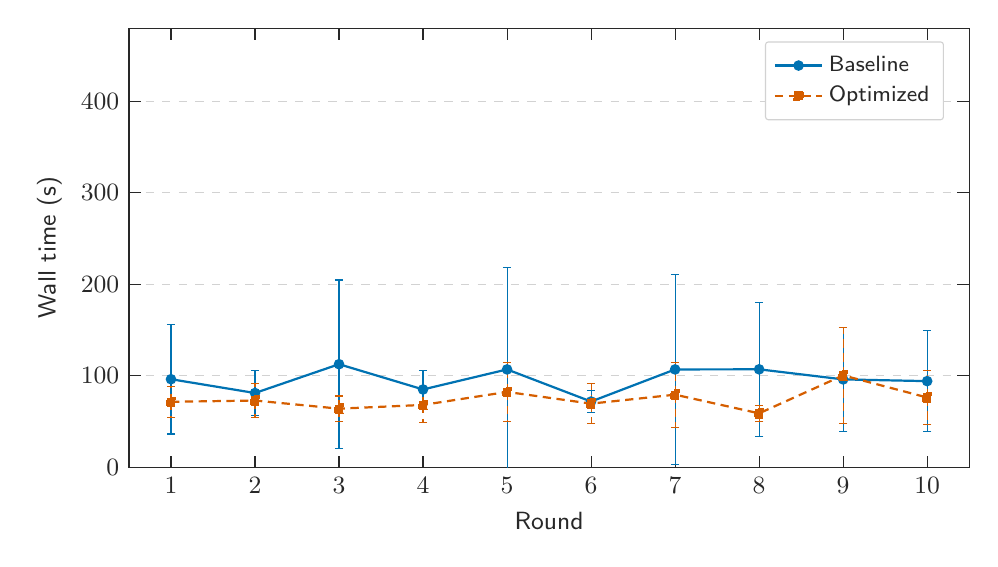
\begin{tikzpicture}
\begin{axis}[
  fcstyle,
  xlabel={Round},
  ylabel={Wall time (s)},
  xtick={1,2,...,10},
  ymin=0, ymax=480,
  xmin=0.5, xmax=10.5,
  legend pos=north east,
]
\addplot[color=clrAcc, thick, mark=*, mark size=1.5pt,
         error bars/.cd, y dir=both, y explicit] coordinates {
  (1,96.4)  +- (0,59.9)
  (2,81.3)  +- (0,24.7)
  (3,112.8) +- (0,92.0)
  (4,85.2)  +- (0,20.8)
  (5,107.1) +- (0,111.4)
  (6,72.0)  +- (0,12.2)
  (7,107.1) +- (0,103.9)
  (8,107.2) +- (0,73.2)
  (9,96.2)  +- (0,56.8)
  (10,94.3) +- (0,55.2)
};
\addlegendentry{Baseline}
\addplot[color=clrLoss, thick, mark=square*, mark size=1.5pt,
         densely dashed,
         error bars/.cd, y dir=both, y explicit] coordinates {
  (1,71.7)  +- (0,16.8)
  (2,73.1)  +- (0,18.8)
  (3,64.2)  +- (0,13.9)
  (4,68.3)  +- (0,18.8)
  (5,82.5)  +- (0,31.9)
  (6,69.7)  +- (0,21.8)
  (7,79.5)  +- (0,35.5)
  (8,59.1)  +- (0,9.0)
  (9,100.6) +- (0,52.7)
  (10,76.4) +- (0,29.1)
};
\addlegendentry{Optimized}
\end{axis}
\end{tikzpicture}
\caption{Mean round wall time $\pm1$\,std per round index ($n=10$
  sessions). Baseline error bars reflect blocking IPFS upload spikes.
  The optimized variant eliminates these spikes from the critical path.}
\label{fig:walltime}
\end{figure}

Transaction confirmation accounts for the baseline mean of 58.5\,s
(optimized: 37.3\,s; see Table~\ref{tab:overhead}) and is the floor below which no round can fall
regardless of optimization. The 21.2\,s confirmation improvement in the
optimized variant is attributed to lower mean Base~L2 network congestion
during the later experiment window rather than any code change, as
confirmation is entirely external to the client. The 22.4\% mean reduction
and 57.6\% std reduction are both attributable to O3 alone; O1+O2+O4
contribute a further $\approx$2.0\,s deterministic saving per round.

\subsection{Audit Trail Reliability and Cost Analysis}
\label{subsec:cost}

Tables~\ref{tab:audit_stats} and~\ref{tab:costs} report the blockchain audit
statistics and cost analysis for the full 200-round experiment. Over 840
pin-map entries spanning 20 sessions, 97.1\% of IPFS pins succeeded; all 24
soft failures were retried automatically and the CIDs remain pinned and
accessible. Model payload bytes are bit-identical at 3{,}439{,}144 bytes
across all 200 rounds, confirming reproducible SE-ResNet serialisation under
PyTorch~2.3 on ARM Cortex-A72 hardware. Most significantly, \texttt{verifyChain()}
returned \texttt{true} in all 20 sessions with zero hash violations, providing
a cryptographic guarantee that no historical on-chain record was tampered with
across the entire experiment.

\begin{table}[t]
\caption{Blockchain audit infrastructure statistics (20 sessions, 200 rounds).}
\label{tab:audit_stats}
\centering\footnotesize
\setlength{\tabcolsep}{4pt}
\begin{tabular}{lr}
\toprule
\textbf{Metric} & \textbf{Value} \\
\midrule
Sessions (baseline\,/\,optimized) & 10\,/\,10 \\
Total FL rounds (excl.\ R0) & 200 \\
On-chain transactions total & 620 \\
Blocks written per session (1~init $+$ 3$\times$10) & 31 \\
Cumulative chain blocks & 1{,}862 \\
\midrule
IPFS pin entries (tx\_pin\_map.csv) & 840 \\
Pin types: GLOBAL\,/\,LOCAL\,/\,VOTE & 440\,/\,200\,/\,200 \\
Pin success (baseline) & 410\,/\,420 (97.6\,\%) \\
Pin success (optimized) & 406\,/\,420 (96.7\,\%) \\
Pin success (overall) & 816\,/\,840 (97.1\,\%) \\
Unique IPFS CIDs pinned & 760 \\
Model payload (gzip, bytes) & 3{,}439{,}144 \\
Model payload std across 200 rounds & 0 (bit-identical) \\
\texttt{verifyChain()} violations & 0\,/\,20 sessions \\
\bottomrule
\end{tabular}
\end{table}

\begin{table}[t]
\caption{Three-way cost comparison. ETH\,=\,\$2{,}300 (April~2026 spot).
  L1 per-round cost: $260{,}000$\,gas $\times$ 40\,gwei $\times$ \$2{,}300\,=\,\$23.9.}
\label{tab:costs}
\centering\footnotesize
\setlength{\tabcolsep}{3pt}
\begin{tabular}{lrrr}
\toprule
\textbf{Metric} & \textbf{ETH L1 (est.)} & \textbf{Base L2 Baseline} & \textbf{Base L2 Opt.} \\
\midrule
Cost per TX             & \$9--\$50       & $<$\$0.004    & $<$\$0.004 \\
Cost per round (3 TX)   & $\approx$\$24   & $<$\$0.012    & $<$\$0.012 \\
Cost per session        & $\approx$\$240  & $<$\$0.12     & $<$\$0.12 \\
Total (200 rounds)      & $\approx$\$4{,}800 & $<$\$2.48  & $<$\$2.48 \\
\midrule
Mean wall time/round    & ---             & 96.0\,s       & 74.5\,s \\
Wall time std           & ---             & 67.3\,s       & 28.5\,s \\
Rounds per hour         & ---             & 37.5          & 48.3 \\
\midrule
vs.\ L1 (min \$24/rnd)  & 1$\times$       & $>$\textbf{2{,}000}$\times$ & $>$\textbf{2{,}000}$\times$ \\
vs.\ L1 (med.\ \$67/rnd)& 1$\times$       & $>$\textbf{5{,}583}$\times$ & $>$\textbf{5{,}583}$\times$ \\
\bottomrule
\end{tabular}
\end{table}

The $>$2{,}000$\times$ minimum cost reduction (using the lowest plausible
L1 estimate of \$24/round at \$2{,}300 ETH and 40\,gwei) and
$>$5{,}600$\times$ reduction at median L1 rates are not minor engineering
conveniences: at L1 rates, the equivalent 200-round experiment would cost
\$4{,}800--\$30{,}000, making iterative research economically infeasible.
At L2 rates, the blockchain record costs less than a cup of coffee per
session and under \$0.012 per aggregation round regardless of the number
of clients or model size. The cost per TX is fixed, so FLBL2's audit
overhead does not grow with model parameters, dataset size, or number of
training examples---only with the number of rounds and TX types per round.


\FloatBarrier
% ============================================================
\section{Security Analysis}
\label{sec:security}

Table~\ref{tab:threats} summarises the threat model. FLBL2 provides
\emph{audit trail integrity}: any party can confirm that the published
global model matches the on-chain CID and that the CID chain has not
changed since commitment. It does not provide Byzantine fault tolerance
during training; the voting mechanism is informational only.

\begin{table}[h]
\caption{Threat model.}
\label{tab:threats}
\centering\footnotesize
\setlength{\tabcolsep}{3pt}
\begin{tabular}{p{2.8cm}p{3.8cm}p{3.4cm}}
\toprule
\textbf{Threat} & \textbf{FLBL2 mechanism} & \textbf{Residual risk} \\
\midrule
Aggregation tampering &
  CID committed on-chain; \texttt{verifyChain()} detects hash breaks &
  Requires server key compromise \\
Gradient poisoning~\cite{blanchard2017machine,fang2020local} &
  Vote record flags high-loss clients; audit-only &
  Does not block poisoning \\
Inference attacks on artifacts &
  Weights on IPFS are intentionally public; raw data stays on-device &
  By design; no raw data leaves devices \\
IPFS unavailability &
  Pinata SLA; CID committed on-chain permanently &
  Prolonged outage loses artifact, not commitment \\
Smart contract exploit &
  OpenZeppelin Ownable+Pausable; owner-only writes; Solidity~0.8 checked arithmetic &
  Server key management risk \\
Privacy of metadata &
  Loss values and CIDs are public; no raw data on-chain &
  Round-level stats are public by design \\
\bottomrule
\end{tabular}
\end{table}

Byzantine-robust aggregation~\cite{blanchard2017machine} and
poisoning-resistant FL~\cite{fang2020local,dong2024defending} address the
gradient-poisoning residual risk, but are orthogonal to our audit
contribution; they can be composed with FLBL2 without modifying the
on-chain record structure. A comprehensive FL security survey by Li et
al.~\cite{li2023security} classifies attacks on data, model, and
infrastructure layers and finds that immutable audit trails mitigate a
subset of data-layer attacks by enabling post-hoc forensics, even when
Byzantine filtering fails.

For deployments where per-round training statistics are sensitive, loss
values in the vote record could be replaced by homomorphic commitments or
zero-knowledge proofs of correct aggregation, at the cost of additional
computation and higher gas per transaction.


\FloatBarrier
% ============================================================
\section{Discussion}
\label{sec:discussion}
In this section, we discuss the practical implications of the proposed FLBL2 framework, including its scalability, deployment feasibility, and applicability to real-world edge and IoT scenarios. We also examine current limitations, such as reliance on centralized pinning services and assumptions in the threat model, and outline promising directions for future work, including decentralized storage alternatives, enhanced security mechanisms, and broader validation across heterogeneous environments.

\subsection{Practical Significance and Dataset Contribution}
The primary result is straightforward: a per-round blockchain audit of a physical FL deployment is now cheap enough to do by default. At
${<}\$0.012$/round on Base~L2, cost is no longer the obstacle. The
system ran 200 rounds across 20 sessions without a single on-chain
write failure or verification error. All 24 soft IPFS pin failures (2.9\% of 840
attempts) were retried automatically and all CIDs remain accessible, demonstrating
that a full audit trail is operationally feasible on commodity edge
hardware at the scale of a real FL experiment.

The $57.6\%$ variance reduction from O3 is practically significant for
scheduled FL deployments. High round-time variance makes training sessions
unpredictable in wall-clock time. Moving IPFS uploads off the critical path
addresses the dominant variance source at no cost to FL quality
(Wilcoxon $p=0.103$ for final-round accuracy). The combination of
99.42\% peak accuracy at round~10 and a cost below \$0.13 per session
positions FLBL2 as a production-ready audit layer for healthcare FL
systems~\cite{yazici2023ehealth,singh2022framework,bayan2024blockchain},
where both model quality and traceability are regulatory requirements.
Blockchain-based integrity verification at this cost scale has been shown
viable in educational platforms~\cite{bayan2024blockchain} and IoT
privacy-preserving architectures~\cite{bayan2025permissionless,bayan2025privacy};
the present work extends this to physical FL deployments at 10$\times$ the
scale of prior per-round audit work.

The 200-round experiment produces a publicly released labelled performance
dataset: per-round accuracy, loss, AUC, F1, per-class metrics, per-device
training and evaluation time, CPU, RAM, temperature, the full blockchain
transaction log (block numbers, gas used, confirmation times), and the
840-entry IPFS CID map. To our knowledge, this is the first publicly
available multi-session FL-on-blockchain trace with physical ARM edge
hardware and complete infrastructure telemetry. Prior surveys on FL systems for healthcare~\cite{qammar2023securing} and IoT
applications~\cite{yang2024blockchain,issa2023survey,bayan2025permissionless}
consistently note the absence of reproducible empirical benchmarks;
This dataset addresses that gap directly.

\subsection{Limitations and Future Work}

Pinata is a centralized pinning service; artifact persistence depends on
its SLA. Replacing it with a decentralized alternative
(Filecoin~\cite{protocol2020filecoin}) would improve long-term
availability at the cost of higher integration complexity. The
experiment uses a single aggregation server; a multi-server or
hierarchical aggregation design would test scalability and remove the
single point of trust. The MHEALTH benchmark is near-saturated by
round~7; evaluation on a harder non-IID dataset---for example,
cross-hospital medical imaging~\cite{qu2022blockchain}---would better
stress-test convergence properties under greater data heterogeneity.

Three directions are most promising for future work. First, integrating
a zero-knowledge proof of correct aggregation would let the smart contract
verify aggregation results rather than merely record them, closing the
residual Byzantine gap was identified in the threat model. Second, replacing
equal-weight averaging with stake-weighted or contribution-incentivised
aggregation would align the on-chain record with a reward mechanism,
following the incentive design studied in recent decentralized FL
frameworks~\cite{beltran2026decfl,zhu2026fedERFT,bayan2024privacy}.
Third, evaluating the system with heterogeneous hardware generations
(RPi~3, RPi~4, Jetson~Nano) would characterize performance under the
mixed-device configurations typical of real-world IoT
deployments~\cite{albogamy2025iotfl,minh2025iiot}.


\FloatBarrier
% ============================================================
\section{Conclusion}
\label{sec:conclusion}

\section{Conclusion}

This paper addressed a central accountability gap in federated learning: the lack of a verifiable, tamper-evident training history that can be audited after aggregation has taken place. While FL preserves data locality and reduces direct exposure of private data, it still relies heavily on the integrity of the aggregation process. FLBL2 shows that this limitation can be addressed by combining FL with content-addressed off-chain storage and low-cost public Layer-2 blockchain commitments.

We built, deployed, and benchmarked FLBL2, the first federated learning testbed to achieve full per-round blockchain auditability on real ARM edge hardware using a production Layer-2 mainnet and dual tamper-evidence via both IPFS CIDs and on-chain keccak256 hash chains. The conceptual contribution of FLBL2 is its separation of large model artifacts from compact audit commitments: model-related artifacts are stored off-chain as verifiable IPFS CIDs, while their cryptographic references are committed to an immutable on-chain hash chain. This design makes both artifact tampering and training-history manipulation detectable.

Running on ten Raspberry Pi~4 devices (ARM Cortex-A72, 4\,GB RAM) with production infrastructure, the system achieves 98.6\%$\pm$1.6\% peak accuracy on 12-class wearable HAR across 20 independent sessions, totalling 200 rounds. Blockchain audit costs stay below \$0.012 per round---over 2{,}000$\times$ cheaper than Ethereum~L1 at \$2{,}300/ETH---and all 200 rounds completed with zero on-chain verification failures. These results demonstrate that full per-round auditability is not only technically feasible, but also economically practical for realistic edge-based FL deployments.

The paper also introduced FLBL2-LPSC, a reusable named framework for selecting Layer-2 platforms for FL auditability. By considering transaction cost, finality, compatibility, settlement guarantees, institutional backing, ecosystem maturity, and public accessibility, FLBL2-LPSC frames blockchain backend selection as a core systems design decision rather than a purely implementation-level choice. In addition, the optimized middleware configuration, FLBL2-OPT, reduces mean round time by 22.4\% and variance by 57.6\%, with no effect on FL convergence ($p=0.103$), showing that auditability can be integrated without sacrificing learning quality.

Overall, FLBL2 demonstrates that Layer-2 blockchain makes per-round FL auditability economically routine for production deployment. More broadly, it provides a reproducible model for trustworthy FL infrastructure by combining privacy-preserving distributed learning, verifiable artifact storage, public audit commitments, and cost-efficient blockchain verification.

The full system, logs, and trained models are released at:
\url{https://github.com/shinratttensei1/FLBL2}.

\bibliographystyle{splncs04}
\bibliography{main}

\end{document}
